% !TEX root =  master.tex
%\section{Zieldefinition}
%Das Ziel dieser Arbeit ist es zum einen die Vorteile von Continuous Integration und Continuous Deployment aufzuzeigen und zum anderen verschiedenen Systeme für CI \& CD untereinander zu vergleichen. Das Aufzeigen der Vorteile wird dabei als Aufhänger genutzt um in das Thema einzuleiten. Der Praxisbezug wird durch das Problem der Abteilung hergestellt. Deren CI/CD Pipeline braucht mittlerweile mehr als 20 Minuten um einen Durchlauf abzuschließen. Aus diesem Grund haben Sie sich dazu entschlossen die Pipeline auf einen Cluster aufzuteilen, dabei übernehmen die einzelnen Knoten im Cluster spezialisierte Aufgaben. Ein Knoten kümmert sich zum Beispiel um die Unit-Tests und ein weiterer um Komponententests durchzuführen. Dadurch soll die Zeit für eine Durchlauf reduziert werden. Um diese Cluster aufzubauen gibt es viele Möglichkeiten von vielen Anbietern. Sowohl in der Cloud als auch On Premise. Da die Ressourcen der Abteilung beschränkt sind wollen sie natürlich die am Besten zu ihnen passende Lösung. Mit dieser Problemstellung wird sich diese Arbeit größtenteils beschäftigen. Am Ende der Arbeit soll eine Handlungsempfehlung für die Abteilung vorliegen an der sie sich orientieren kann.
%\section{Untersuchungsmethodik}
%Damit die Alternativen möglichst objektiv bewertet werden können soll eine AHP-Analyse(Analytic Hierarchy Process) durchgeführt werden. Dabei ist das Ziel möglichst viele Stakeholder an der Aufstellung des Kriterienkatalogs und der Gewichtung teilhaben zu lassen.
\chapter{Einleitung}
\begin{center}\textbf{\enquote{Das muss man doch auch automatisieren können!?}}\end{center}
So oder so ähnlich muss es jedem Entwickler oder auch Administrator schon einmal durch den Kopf gegangen sein. Sei es bei einfachen repetitiven Aufgaben wie zum Beispiel das Anlegen eines neuen Users, oder auch beim Administrieren von großen Serverclustern. Und damit haben sie auch Recht. Mittlerweile gibt es unzählige Tools, die genau solche Aufgaben auf einfache Art und Weise automatisieren können.\\
Doch warum dort mit der Automatisierung stoppen?\\
Schon während der Entwicklung lassen sich viele Schritte automatisieren. Dies steigert die Geschwindigkeit des Entwicklungsprozesses und schont die Nerven der Entwickler.
\section{Motivation}
Möglich gemacht wird dies durch sogenannte Continuous Practices (\ac{CI}, \ac{CDE} und \ac{CD}) (siehe \ref{CP}). Sie helfen dem Entwickler(-team) dabei, ihre Entwicklungen zu \enquote{bauen}, zu testen und falls es entsprechend konfiguriert ist, auch zu veröffentlichen beziehungsweise auf entsprechenden Systemen zu installieren.\\ Dies steigert die Flexibilität und Agilität der Entwickler und verkürzt die Time-to-Market (also die Zeit, die gebraucht wird, um von der Entwicklung zum fertigen und releasefähigem Produkt zu kommen). Sie können sich viel besser auf die tatsächliche Entwicklung konzentrieren anstatt auf die Aufgaben, die nebenbei getätigt werden müssen.\\ Trotz dieser Vorteile sind Continuous Practices nicht so weit verbreitet, wie man annehmen würde. Laut einer Umfrage (\cite{JetBrains.2016}) benutzten erst 44\% der Entwickler weltweit diese Practices tatsächlich während der Entwicklung.\autocite[Vgl.][]{JetBrains.2016}  Damit bleibt eine Menge Potential ungenutzt. Viele Unternehmen geben an, dass ihnen geschulte Mitarbeiter für diese Technologien fehlen, außerdem fehlt ihnen schlichtweg die Zeit, um die Prozesse zu automatisieren.\autocite[Vgl.][]{Claranet.2016}\\ Aus diesem Grund möchte die Abteilung \ac{CAP} ein Angebot für \ac{CI}/\ac{CDE}/\ac{CD} as a Service erstellen. \enquote{as a Service} bedeutet dabei, dass der Kunde kein eigenes dediziertes System mehr erhält. Stattdessen bezahlt er für die Bereitstellung eines Services in der Cloud. Er bezahlt dabei nur für die Nutzung und nicht das gesamte System. Des Weiteren sind solche Systeme sehr gut skalierbar. Das bedeutet, dass der Kunde bei erhöhtem Leistungsbedarf diese Mehrleistung sehr schnell erhalten kann, ohne dass große Umstellungen getätigt werden müssen.\\ Die Abteilung möchte dem Kunden (intern sowie extern) damit ein möglichst komplettes \ac{CI}/\ac{CDE}/\ac{CD} System bieten, auf dem der Kunde so wenig wie möglich anpassen muss. Vom Hosting bis zu etwaigen Integration von Projekten soll alles angeboten und übernommen werden. Es soll eine gesamte konfigurierte Entwicklungsplattform angeboten werden.
\section{Problemstellung} 
Wie fängt man bei der Erstellung eines Angebots für \ac{CI}/\ac{CDE}/\ac{CD} as a Service an? Damit man überhaupt etwas anbieten kann, braucht man zunächst einen Service. Doch wie zieht man diesen Service auf? Man kann das komplette System mitsamt \ac{CI}/\ac{CDE}/\ac{CD}-Tools von Grund auf aufbauen. Allerdings würde dies nur extra Arbeit schaffen. Mittlerweile gibt es unzählige Tools für \ac{CI}, \ac{CDE} und \ac{CD} am Markt. Viele davon sind spezialisiert auf besondere Anwendungsgebiete, aber es gibt auch einige Allrounder.\\ Doch welches Tool ist jetzt das am besten geeignete für die Anwendung in dem Service? Und wie wähle ich das am besten geeignete Tool aus?\\
Mit diesen Problemstellungen wird sich diese Arbeit im Folgenden beschäftigen. Es wird ein Analyseverfahren ermittelt mithilfe dessen dann verschiedene Alternativen evaluiert werden.
Ziel dieser Bachelorarbeit ist es, verschiedene \ac{CI}/\ac{CDE}/\ac{CD}-Tools zu evaluieren, um am Ende der Abteilung ein Tool präsentiert zu können, welches mit den Anforderungen der Abteilung am besten übereinstimmt. Die Anforderungen der Abteilung werden vorher erarbeitet und mithilfe eines geeigneten Analyseverfahrens entsprechend ihrer Prioritäten aufgenommen. Dabei werden möglichst viele Stackeholder in den Prozess mit einbezogen, um am Ende ein möglichst objektives Ergebnis zu erhalten.\\
\\
Der Fokus der Arbeit liegt dabei auf dem analytischen Vergleich der verschiedenen Alternativen, welche zuvor eine Vorauswahl durchlaufen, da der Vergleich aller Tools den Rahmen dieser Arbeit sprengen würde. Die Implementierung des \ac{CI}/\ac{CDE}/\ac{CD} as a Service ist kein Teil dieser Arbeit. Des Weiteren  soll mit der Arbeit ein Einblick in das \ac{CI}, \ac{CDE} und \ac{CD} \enquote{Ökosystem} gegeben werden, um damit einen Erkenntnisgewinn für die Abteilung zu erhalten.
\section{Vorgehensweise}
Zu Beginn der tatsächlichen Arbeit werden zuerst die informationstechnischen Grundlagen geschaffen. Sowohl Continuous Practices als auch Versionsverwaltungssysteme werden als eingesetzte Technologien erklärt. Danach werden drei verschiedene analytische Vergleichsmethoden vorgestellt und die passendste Methodik für die Problemstellung ausgewählt. Mithilfe dieser Analysemethode werden dann vier zuvor evaluierte \ac{CI}/\ac{CDE}/\ac{CD}-Tools anhand verschiedener Kriterien verglichen. Das Ergebnis dieser Analyse wird als Grundlage für eine Handlungsempfehlung genutzt, die dann im weiteren Verlauf ausgesprochen wird. Am Ende findet noch eine Zusammenfassung der Ergebnisse und Erkenntnisse statt. Sie werden noch einmal komprimiert dargestellt und kritisch reflektiert. Zum Schluss wird darüber hinaus noch ein Ausblick auf mögliche weitere Entwicklungen nach Beendigung der Arbeit gegeben.
\chapter{Informationstechnische Grundlagen} 
Im folgenden Abschnitt werden die informationstechnischen Grundlagen geschaffen, die für das Verständnis dieser Arbeit relevant sind. Hierfür werden sowohl Continuous Practices als auch Versionsverwaltungssysteme erläutert. Des Weiteren wird DevOps als Methodik zur Verbindung von Continuous Practices und agiler Arbeitsweise erläutert.
\section{Versionsverwaltungssysteme}\label{vcs}
In der heutigen Softwareentwicklung besteht ein Projekt aus vielen Quellcode-Dateien, die ständig neu erstellt und verändert werden. Um jegliche Veränderungen an dem Quellcode zu dokumentieren und nachvollziehen zu können, wird ein Versionskontrollsystem (Version Control System; VCS) genutzt.\autocite[Vgl.][S.6]{Baerisch.2005}  
Dieses ermöglicht es dem Entwickler beispielsweise, Weiterentwicklungen durchzuführen, während parallel an der aktuellen Version Fehler behoben werden. Darüber hinaus erlaubt eine Versionsverwaltung dem Entwickler, Änderungen mit anderen zu teilen und Änderungen von verschiedenen Personen zusammenzuführen.\autocite[Vgl.][S.9]{Kleine.2012} \\
Ein VCS bietet die Möglichkeit, Änderungen von Informationen beispielsweise an einem Quellcode zu organisieren und zu verwalten. \autocite[Vgl.][S.1]{Pilato.2009}
Die wachsende Sammlung an Informationen dient als „Repository (Lager), Projektgeschichte, Kommunikationsmedium und Werkzeug zur Team- und Produktverwaltung“.\autocite[][S.1]{Loeliger.2010} In einer Versionsverwaltung lagern somit nicht nur die Quelldateien, sie dient auch als Kernstück für ein ganzes Entwicklungsprojekt. \\
Zentrale Aufgaben der Versionsverwaltung sind der Zugriff auf historische Versionen der Dateien, Aufzeichnung der Änderungen in einem Log und die Entwicklung und Pflege eines Repository mit Inhalten. Die Aufbewahrung von älteren Versionen ist gerade in der Softwareentwicklung wichtig, da Software nach dem „Probierprinzip“\autocite[][S.9]{Versteegen.2003} entwickelt wird. Auf eine neue Entwicklung folgt ein anschließender Test. Es werden so lange Anpassungen durchgeführt und getestet, bis das optimale Ergebnis erreicht wurde.\autocite[Vgl.][S.9]{Versteegen.2003}
Ein Tool zur Sourcecodeverwaltung ermöglicht zudem das Management von Änderungen und den Zugriff von mehreren Entwicklern am gleichen Projekt.\autocite[Vgl.][S.1]{Loeliger.2010} Dies fördert die Zusammenarbeit an einem Projekt, da parallel unterschiedliche Entwicklungen von mehreren Personen getätigt werden können. Gerade bei der Arbeit in einem Team muss die Möglichkeit der parallelen Entwicklung gegeben sein, da sich sonst die Entwickler in ihrer Arbeit gegenseitig beeinträchtigen.
\section{Continuous Practices}\label{CP}
Wie bewältigt man die größer werdende Nachfrage von Unternehmen und dem eigenen Management nach kürzerer Time-to-Market (also der Zeit von der Entwicklung bis zum fertigen Produkt) und einer erhöhten Flexibilität und Agilität bei der Entwicklung?\autocite[Vgl.][]{Capgemini.2017}\\ Continuous Integration, Continuous Delivery und Continuous Deployment (Auch Continuous Practices genannt) sind Techniken, um genau diesen Prozess zu unterstützen.  Sie bieten die Möglichkeit, die Geschwindigkeit des Entwicklungsprozesses zu erhöhen, ohne Qualität einzubüßen.\autocite[Vgl.][S.2]{Shahin.2017}
Die Idee hinter Continuous Integration ist dabei nicht sonderlich neu. Bereits in den 90er Jahren wurde die Idee im größeren Kontext von Extreme Programming und dem Agilen Manifest erwähnt.\autocite[Vgl.][S.2]{Stahl.2018} Auch die grundlegende Idee, eine große Aufgabe in viele kleine Teile zu zerlegen und diese dann einzeln zu bearbeiten, ist nicht neu.\\ Über die Jahre hat sich die Idee weiterentwickelt und wurde von immer mehr Entwicklerteams aufgegriffen. Später kamen dann noch Continuous Delivery und Continuous Deployment hinzu, die mithilfe von Automatisierung den Prozess weiter ausbauten und beschleunigten. Die Abgrenzung zwischen den Begriffen ist dabei nicht genau definiert, weswegen für viele zum Beispiel Teile der Continuous Delivery noch zu Continuous Integration gehören und für andere wiederum nicht. Insgesamt sollen aber alle Continuous Practices zu positiven Veränderungen führen:\autocite[Vgl.][S.2]{Shahin.2017}
\begin{itemize}
	\item Häufigeres und schnelleres Feedback aus dem Entwicklungsprozess und vom Kunden selbst 
	\item Erhöhte Releasezyklen mit stabilen Produkten führt zu erhöhter Produktqualität und verbesserter Kundenzufriedenheit
	\item Manuelle Aufgaben werden automatisiert
\end{itemize}
Im Folgenden wird nun auf die drei Hauptpractices im Detail eingegangen: Continuous Integration, Continuous Delivery und Continuous Deployment. Es existieren noch einige weitere Begriffe, allerdings sind die drei am bekanntesten und sind dementsprechend am häufigsten im Einsatz. Ihre Funktionen werden beschrieben und von dem abgegrenzt was sie nicht sind. 
\subsection{Continuous Integration}
Continuous Integration ist wohl die bekannteste aller Practices und wird immer wieder als Synonym für alle Continuous Practices genannt.\autocite[Vgl.][S.12]{Stahl.2018} Dabei ist es per Definition nur \enquote{eine Softwarenetwicklungspraktik, bei der Entwickler, aus einem Team, ihre Veränderungen häufig in das Projekt integrieren. Mindestens einmal täglich}\autocite[S.12]{Stahl.2018}\\
Dies ist wichtig wenn die Größe des Entwicklungsteams über 1 wächst. Denn sobald mehrere Leute an einem Projekt arbeiten, wird es schwieriger, die Veränderungen des einen Entwicklers mit denen des anderen zu verknüpfen und das Programm zum Laufen zu kriegen.\autocite[Vgl.][S.4]{Stahl.2018}\\ Man kann es vergleichen mit dem gemeinsamen Schreiben vieler Autoren an einem sehr langen Roman. Die Geschichte und alle Charaktere müssen konsequent geschrieben sein, damit das Buch verständlich ist. Je mehr Autoren mitarbeiten, umso schwieriger wird es, die einzelnen Teile zusammenzuführen.\\ Das gleiche Problem tritt auch in der Softwareentwicklung auf und wird komplizierter mit jedem Entwickler, der dazu kommt. Außerdem wird es umso schwieriger, wenn Veränderungen von einem Entwickler länger zurückgehalten werden. Je umfangreicher die Veränderungen sind, die eingebracht werden, umso schwieriger wird es, diese zu integrieren.\\ Dies bringt uns wieder zur Definition vom Anfang. Es geht nicht darum, so oft und schnell wie möglich zu integrieren, sondern um die Häufigkeit und Regelmäßigkeit.\autocite[Vgl.][S.3]{Stahl.2018} Darüber hinaus werden die Veränderungen automatisch getestet, um eine sichere Basis zu haben, auf der alle arbeiten können.\\ Continuous Integration führte zu einem Paradigmenwechsel. Ohne Continuous Integration ist die Applikation nicht lauffähig, bis das Gegenteil in Form von Tests oder dem Deployment bewiesen ist. Mit Continuous Integration funktioniert die Applikation erwiesenermaßen (Automatische Builds, Tests etc.). Und es wird sofort bemerkt, wenn etwas nicht mehr funktioniert.\autocite[Vgl.][S.40]{Farley.2010}\\ Es beschleunigt den gesamten Entwicklungsprozess, da weniger Ressourcen für das Integrieren gebraucht werden. Des Weiteren bildet Continuous Integration die Grundlage für Continuous Delivery und Continuous Deployment. Ohne kontinuierliches Integrieren bringen diese beiden Practices keinen Vorteil.\autocite[Vgl.][S.7]{Stahl.2018}
\subsection{Continuous Delivery}
2010 haben Jez Humble und David Farley\autocite{Farley.2010} die Idee der Continuous Integration weiterentwickelt. Sie gehen von der Basis, welche durch die Veränderungen der Entwickler regelmäßig gepflegt wird, aus, und behandeln jede Bearbeitung dieser Basis als möglichen Releasekandidaten.\autocite[Vgl.][S.5]{Stahl.2018} Mithilfe einer automatisierten Pipeline, also einer Abfolge von Programmausführungen auf die Codebasis, wird aus dem Code ein lauffähiges Programm. Das Ziel dieses Prozesses ist es, immer einen lauffähigen und getesteten Releasekandidaten zu haben, welcher bei Bedarf, zum Beispiel um dem Kunden den Fortschritt zu zeigen, manuell deployed oder auch released werden kann.\autocite[Vgl.][S.16]{Stahl.2018}
\begin{figure}[h!]
	\centering
	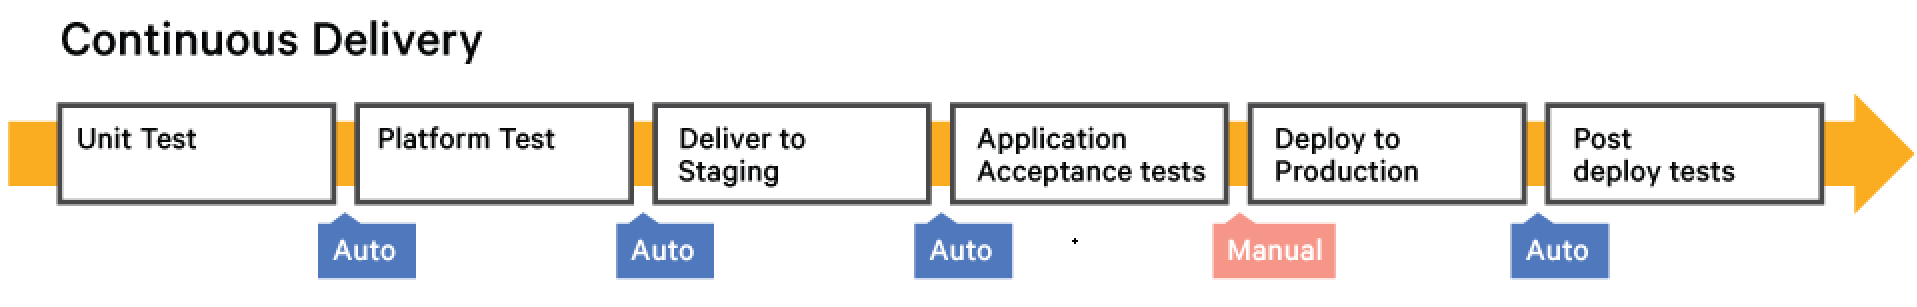
\includegraphics[scale = 0.3]{img/CDE.png}
	\quelle{\cite{Puppet.2013}}
	\caption{Continuous Delivery Pipeline}
	\label{img:cde}
\end{figure}\\
In Abbildung \ref{img:cde} findet sich eine auf das wesentliche herunter gebrochenen Beispielpipeline. Dabei fehlt der wichtige erste Schritt aus Continuous Integration: das tatsächliche Integrieren.\\ Hier stoßen wir bereits auf die erste Technologie. Damit das Integrieren von vielen Veränderungen von verschiedenen Entwicklern gleichermaßen geordnet und protokolliert abläuft, wird heutzutage vermehrt ein Versionsverwaltungssystem (\ref{vcs}) genutzt.\autocite[Vgl.][S.2]{Arachchi.2018} Dort wird der gesamte Code zentral verwaltet und bildet damit die beschriebene Basis für die weiteren Vorgänge. Des Weiteren dient es auch als Auslöser zum Start der gesamten Pipeline. Veränderungen werden automatisch vom System erkannt, welches dann die automatische Pipeline anstößt. Bei dem System handelt es sich meistens um einen dedizierten CI/CD Server, welcher die Pipeline dann entsprechend ihres Aufbaus abarbeitet.\autocite[Vgl.][S.2]{Meyer.2014}\\ Noch vor dem ersten Schritt aus Abbildung \ref{img:cde} wird die Applikation erst einmal gebaut. Das heißt, etwaige Abhängigkeiten werden installiert, und der Quellcode wird in einen ausführbaren Programmcode übersetzt.\autocite[Vgl.][S.36]{Farley.2010} Des Weiteren wird mit diesem Schritt auch der erste Test der Applikation durchgeführt. Wenn die Syntax des Quellcodes nicht stimmt, würden hier die ersten Fehler auftreten.\autocite[Vgl.][S.37]{Farley.2010}\\ Theoretisch fallen diese Schritte noch in den Bereich von Continuous Integration. Sie werden erst hier beschrieben, damit ein Gesamtbild über den Ablauf gegeben werden kann.\\
Nachdem die Applikation gebaut ist, kann sie getestet werden. Hierfür können verschiedene automatisierte Testverfahren eingesetzt werden.
\begin{itemize}
	\item \texttt{Unit-Tests(Komponententests)} \\Unit-Tests überprüfen, ob die von den Entwicklern geschriebenen Komponenten so arbeiten, wie diese es beabsichtigen. Zum Beispiel ob ein Input den gewünschten Output liefert.\autocite[Vgl.][S.21]{Westphal.2012} Zur Qualitätssicherung wird eine sehr häufige Ausführung der Komponententests angestrebt. Dabei ist es üblich, dass der Test in der gleichen Sprache wie das Testobjekt geschrieben wird.
	\item  \texttt{Statische Codeanalyse}\\ \enquote{Die statischen [Code]Analyseverfahren [dienen der] Syntax-, Konsistenz- und Vollständigkeitsprüfung.}\autocite[S.264]{Bommer.2008} Statische Tests sorgen dafür, dass Fehler und potenzielle Fehlerquellen frühzeitig erkannt werden. Dabei steht die Prävention von Fehlern im Vordergrund. Sie sollen so früh wie möglich erkannt werden, um spätere und arbeitsintensive Nachbesserungen zu vermeiden.\autocite[Vgl.][S.263]{Bommer.2008}
	\item  \texttt{End-to-End Tests} \\End-to-End Tests werden genutzt, um Abläufe innerhalb einer Applikation vom Anfang bis zum Ende zu testen. Der Zweck von End-to-End Tests ist dabei die Simulation von echten Nutzerszenarien und die Validierung des Systems und der Datenintegrität.\autocite[Vgl.][S.250]{Bommer.2008} Dabei werden Szenarien aus der echten Welt getestet, wie zum Beispiel die Kommunikation über die API, die Kommunikation mit der Datenbank und vieles mehr. End-to-End Tests sind dabei sehr arbeitsintensiv, weil bei Änderungen zum Beispiel an der Weboberfläche auch alle End-to-End Tests überarbeitet werden müssen. Diese würden sonst fehlschlagen.\autocite[Vgl.][S.252]{Bommer.2008}
\end{itemize}
 Sollten ein oder mehrere Tests fehlschlagen, wird dies auf dem CI/CD System angezeigt, und der Entwickler kann entsprechende Fehler leicht erkennen und ausbessern. Des Weiteren werden alle eventuell schon installierten Teile auf die Ausgangsbasis zurück gerollt um etwaige Beeinträchtigungen zu vermeiden. Wenn die Veränderung also auf das Entwicklungssystem ausgerollt wird und während des Durchlaufs der Pipeline ein Fehler auftritt, dann werden alle gemachten Veränderungen verworfen, und das System kann ganz normal weiter funktionieren.\autocite[Vgl.][S.41]{Farley.2010} Wenn alle Tests positiv verlaufen sind, wird die Pipeline fortgeführt.\\
 Der nächste Schritt wäre die Implementierung der getesteten Applikation auf einer sogenannten Staging Umgebung. Dort sind dieselben Voraussetzungen gegeben wie auf der späteren Produktivumgebung.\autocite[Vgl.][S.283]{Farley.2010} Dort kann der Kunde sich die gemachten Veränderungen anschauen und überprüfen. Die Abnahme, also die Bestätigung, dass die Veränderung mit den Interessen des Kunden übereinstimmen, (auch Acceptance Tests genannt) kann entweder manuell oder automatisiert geschehen. Bei manueller Abnahme ist der Arbeitsaufwand ungemein höher, weil bei jeder integrierten Veränderung eine Abnahme gemacht werden muss. Mit automatisierten Acceptance Tests wird der gesamte Prozess beschleunigt und Kosten gespart.\autocite[Vgl.][S.310]{Farley.2010} Acceptance Tests werden ähnlich wie End-to-End Test aufgebaut, um die Usererfahrung abzubilden. Dabei werden die Tests meistens direkt auf dem User Interface ausgeführt. Am Erstellen dieser Tests sind meistens alle Stackeholder der Applikation beteiligt, vom Entwickler bis zum Kunden.\autocite[Vgl.][S.312]{Farley.2010}\\
 Dabei sind die Testfälle immer gleich aufgebaut\autocite[Vgl.][S.312]{Farley.2010}:
 \begin{itemize}
 	\item\textbf{GIVEN} some initial context,
 	\item\textbf{WHEN} an event occurs,
 	\item\textbf{THEN} there are some outcomes.
 \end{itemize}
Es wird der Input, die aufgerufene Aktion und das gewünschte Ergebnis beschrieben. Mit dieser Syntax lassen sich alle Testfälle beschreiben.\autocite[Vgl.][S.312]{Farley.2010}\\
Sobald die Acceptance Tests erfolgreich durchgeführt sind, endet die automatische Pipeline. Am Ende steht eine releasefähige Version der Applikation, welche ausreichend getestet und abgenommen wurde. Da die Pipeline bei jeder Veränderung ausgelöst wird, hat man also immer ein aktuelle lauffähige Version, die jederzeit präsentiert oder auch released werden kann. Dem Rollout auf das Produktivsystem steht jetzt hoffentlich nur noch ein Knopfdruck im Weg, wenn der Deploymentprozess entsprechend automatisiert ist. Wenn der Kunde oder das Management dann die Freigabe zum Release erteilt, geht alles ganz schnell.\autocite[Vgl.][S.289]{Farley.2010}
\subsection{Continuous Deployment}
Continuous Deployment geht noch einen Schritt weiter und sagt:\enquote{Jede Veränderung soll direkt auf das Produktivsystem deployed werden}\autocite[Vgl.][S.17]{Stahl.2018} Damit automatisiert Continuous Deployment den letzten Schritt, den Continuous Delivery als manuelle Tätigkeit übrig lässt (siehe Abbildung \ref{img:cde2}).
\begin{figure}[h!]
	\centering
	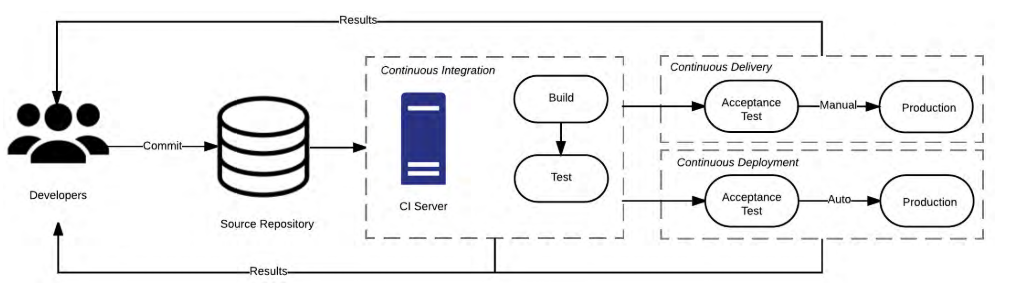
\includegraphics[scale = 0.6]{img/CDE2.png}
	\quelle{\cite[S.3]{Shahin.2017}}
	\caption{Vergleich Continuous Delivery \& Continuous Deployment}
	\label{img:cde2}
\end{figure}\\
 Wo Continuous Delivery immer einen Releasekandidaten in der Hand hat, welcher jederzeit released werden kann, geht Continuous Deployment diesen Schritt weiter und released jeden Kandidaten.\autocite[Vgl.][S.17]{Stahl.2018} Bevor man allerdings diesen Schritt geht, ist einiges zu beachten. Es sollte darauf geachtet werden, dass es während des Deploymentprozesses zu keinen Downtimes kommt und der Wechsel für den Nutzer praktisch nicht bemerkbar ist. Hierfür kann sich des Blue-Green Deploymentansatzes bedient werden.\autocite[Vgl.][S.407]{Farley.2010}
\begin{figure}[h!]
 	\centering
 	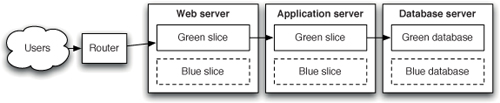
\includegraphics[scale = 1]{img/blue.jpg}
 	\quelle{\cite[S.407]{Farley.2010}}
 	\caption{Blue-Green Deployment}
 	\label{img:blue}
\end{figure}
Bei diesem Ansatz werden zwei Versionen der gleichen Applikation nebeneinander betrieben. Die grüne Applikation (Siehe Abbildung \ref{img:blue}) stellt in diesem Beispiel die alte Version dar, welche zurzeit noch in Betrieb ist. Die blaue Applikation wird währenddessen parallel zur grünen hochgefahren und startbereit gemacht. Sobald die blaue einsatzbereit ist, wird der Traffic von der grünen Applikation auf die blaue gelenkt. Am einfachsten funktioniert dies, wenn dem Ganzen ein Router vorgeschaltet ist, welcher den Traffic lenken kann (siehe Abbildung \ref{img:blue}).\autocite[Vgl.][S.407]{Farley.2010} Für den Nutzer ist der Wechsel kaum spürbar, und die Applikation muss keine Downtime in Kauf nehmen. Außerdem kann im Fall eines Fehlers in der blauen Applikation sofort wieder auf die grüne gewechselt werden. Einzig bei dem Wechsel der Datenbanken kann es zu Komplikationen kommen, da die Daten aus der grünen Applikation auf die Datenbank der blauen kopiert werden müssen.\autocite[Vgl.][S.407]{Farley.2010}\\  
Für den gesamten Prozess des Continuous Deployments ist allerdings zu beachten, dass das Deployment nicht immer so einfach funktioniert. Ein großer Teil der heutzutage eingesetzten Software wird noch vom User selbst installiert, und Veränderungen können nicht so einfach für alle released werden. Mit dem wachsenden Anteil von \enquote{X as a Service}-Angeboten\autocite[S.18]{Stahl.2018} sollte sich dies allerdings bald ändern\autocite[Vgl.][S.18]{Stahl.2018} Allgemein gesagt ist Continuous Deployment also die weitergeführt Idee von Continuous Delivery und hilft dabei, den Prozess weiter zu beschleunigen.
\subsection{DevOps}\label{devops}
Der Begriff DevOps kommt in den letzten Jahren immer häufiger auf\autocite[Vgl.][]{Sauce.2018} und wird dabei auch oft im Zusammenhang mit Continuous Integration, Continuous Delivery und Continuous Deployment genannt. DevOps entstand als Reaktion auf die größer werdende Lücke zwischen der Entwicklung einer Software und dem tatsächlichen Betrieb dieser.\autocite[Vgl.][S.22]{Stahl.2018}\\ Dieser Bewegung schlossen sich immer mehr Leute an, die ihre Erfahrungen mit dem Integrieren von der Entwicklung in die Operations dort einbrachten. Über die Zeit entwickelte sich DevOps weiter, und je bekannter es wurde, umso öfter wurde es mit Continuous Integration, Continuous Delivery und Continuous Deployment genannt und miteinander vertauscht.\autocite[Vgl.][S.23]{Stahl.2018} Im Kern ist DevOps eine Sammlung aus \enquote{Prinzipien, Werten, Methoden und Praktiken}\autocite[S.23]{Stahl.2018}. Zu diesen Praktiken zählen auch Continuous Integration, Continuous Delivery und Continuous Deployment. 
\begin{figure}[h!]
	\centering
	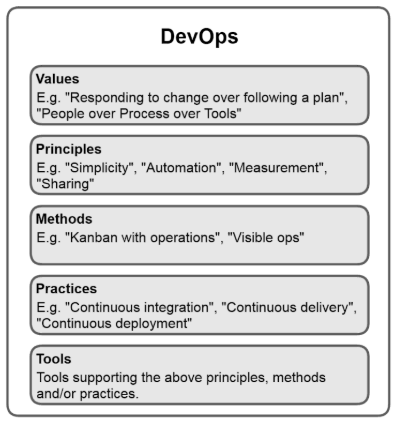
\includegraphics[scale = 0.7]{img/DEVOPS.png}
	\quelle{\cite[S.24]{Stahl.2018}}
	\caption{Zusammensetzung DevOps}
	\label{img:devops}
\end{figure}Diese sowie die anderen Inhalte (siehe Abbildung \ref{img:devops}) von DevOps helfen dabei, die Entwicklung und die Operations miteinander zu verknüpfen und so die allgemeine Zufriedenheit und Produktivität zu verbessern. Dafür muss die sogenannte \enquote{DevOps-Kultur} allerdings erst einmal in allen Ecken eines Unternehmens ankommen.\autocite[Vgl.][S.23]{Stahl.2018} Denn die Implementation von DevOps ist nicht immer einfach. Viele Unternehmen treffen dabei auf Probleme (siehe \cite{Claranet.2016}). Fast 50\% der Unternehmen gaben an, dass die Implementierung an einigen Punkten stockte, aufgrund von mangelnden Qualifikation der Mitarbeiter, fehlender Zeit, und weil es zu Konflikten mit alten Prozessen innerhalb des Unternehmens kam.\autocite[Vgl.][]{Claranet.2016} Wenn DevOps allerdings richtig betrieben wird, ermöglicht es eine Hebelwirkung, die dem gesamten Unternehmen hilft.\autocite[Vgl.][S.24]{Stahl.2018} 
\chapter{Methodische Grundlagen}
Damit der Service erstellt werden kann, muss man sich zuerst für ein \ac{CI}/\ac{CDE}/\ac{CD}-Tool entscheiden. Doch wie entscheidet man sich für eine Alternative? Das folgende Kapitel beschäftigt sich mit der Auswahl der passenden Methodik zur Evaluierung von technischen Alternativen.
\section{Auswahl der vergleichenden Analysemethode}
Mit der Auswahl von Alternativen beschäftigt sich der Forschungsbereich der Entscheidungstheorie. Dort bieten sich verschiedene Methoden an, um Entscheidungen zu treffen. Dabei teilt sich die Entscheidungstheorie in zwei Teilgebiete auf\autocite[Vgl.][S.1]{Laux.2014}:
\begin{itemize}
	\item die präskriptive (normative) Entscheidungstheorie
	\item die deskriptive Entscheidungstheorie 
\end{itemize}
Die deskriptive Entscheidungstheorie beschäftigt sich dabei nur damit, wie und warum Entscheidungen in der Realität getroffen werden. \enquote{Ihr Ziel ist es, empirisch gehaltvolle Hypothesen über das Verhalten von Individuen und Gruppen im Entscheidungsprozess zu finden, mit deren Hilfe bei Kenntnis der jeweiligen konkreten Entscheidungssituation Entscheidungen prognostiziert bzw. gesteuert werden können.}\autocite[S.4]{Laux.2014}\\
Aus diesem Grund wird sich diese Arbeit im Bereich der präskriptiven Entscheidungstheorie bewegen. Es soll nicht herausgefunden werden, wie Entscheidungen gefällt werden, sondern es wird nach einem Modell gesucht, das dabei hilft, rational eine Entscheidung zu treffen. Dafür kommt nur die präskriptive Entscheidungstheorie infrage. Denn \enquote{[sie] will Ratschläge für die Lösung von Entscheidungsproblemen erteilen, also Antwort geben auf die Frage, was ein Entscheider in unterschiedlichen Entscheidungssituationen tun soll.}\autocite[S.4]{Laux.2014} \\
Auch der Bereich der \enquote{\ac{MCDA}} gehört zur präsriptiven Entscheidungstheorie. \ac{MCDA} befasst sich, wie der Name schon aussagt, mit unterschiedlichen Verfahren, die sich dadurch auszeichnen, dass sie kein einzelnes übergeordnetes Kriterium, sondern mehrere unterschiedliche Kriterien nutzen, um Alternativen für die Entscheidungsfindung zu evaluieren. Da in die Entscheidung für ein \ac{CI}/\ac{CDE}/\ac{CD}-Tool viele Kriterien mit einfließen, sind die Verfahren der \ac{MCDA} bestens geeignet, um eine Entscheidung zu treffen und die Alternativen zu evaluieren.\\ \\ Zu den bekanntesten Verfahren gehören:
\begin{itemize}
	\item Nutzwertanalyse
	\item AHP-Analyse (Analytic Hierarchy Process)
	\item TOPSIS (Technique for Order Preference by Similarity to Ideal Solution)
\end{itemize}
Diese drei kommen dabei in die nähere Auswahl für die Anwendung in der späteren Analyse. Alle haben ihre Vor- und Nachteile, die im Folgenden evaluiert werden.
\subsection{Nutzwertanalyse}\label{nutz}
Die Nutzwertanalyse ist besonders in Deutschland, eine bekannte Methode um Alternativen anhand einer Fragestellung zu vergleichen. Dafür wird das Grundproblem/die Fragestellung fragmentiert und in Kriterien umgewandelt.
\begin{figure}[h!]
	\centering
	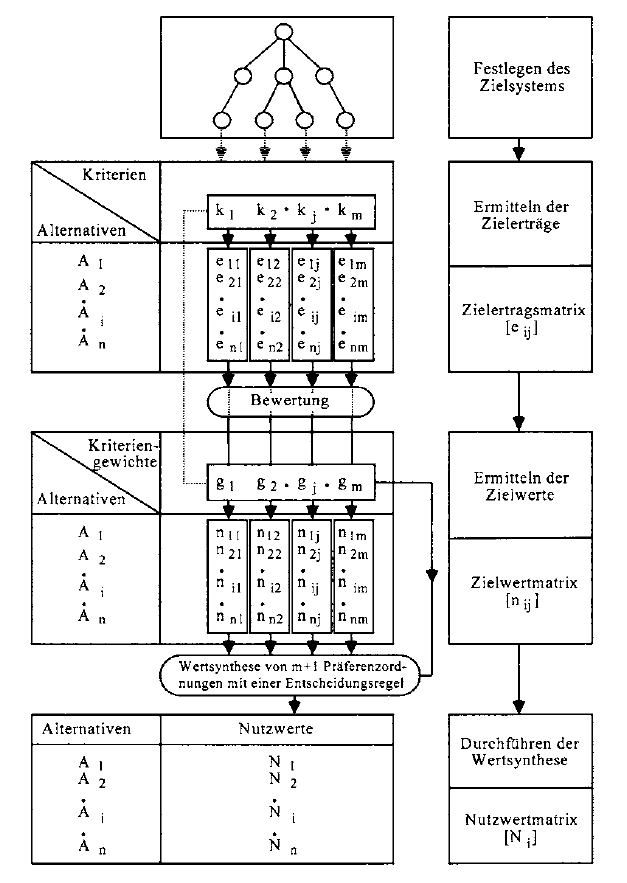
\includegraphics[scale = 0.7]{img/NUTZ.png}
	\quelle{\cite[S.112]{Fink.2006}}
	\caption{Vorgehensweise bei der Nutzwertanalyse}
	\label{img:nutz}
\end{figure}
Diese Kriterien werden gewichtet, und die Alternativen werden im Hinblick auf jedes einzelne Kriterium bewertet.\autocite[Vgl.][S.6]{Kuehnapfel.2014} Am Ende steht eine Gesamtbewertung für jede Alternative, anhand derer die Reihenfolge bestimmt wird (siehe \ref{img:nutz}).\\
Dabei ist die Nutzwertanalyse sehr einfach anzuwenden. Es wird keine große Rechenleistung benötigt, um die Werte auszurechnen. Des Weiteren ist sie einfach erweiterbar. Wenn man also eine Alternative oder ein Kriterium nachträglich hinzufügen will, kann dies ohne große Auswirkungen geschehen.\autocite[Vgl.][S.119]{Fink.2006}\\
Allerdings führt die Einfachheit auch zu Schwachpunkten. Zum Beispiel kann durch die Gewichtung der Kriterien schnell Subjektivität in den Prozess hineinkommen, da sie meistens den größten Einfluss auf das Ergebnis hat. Außerdem ist es nicht möglich, eine Konsistenzprüfung der Daten durchzuführen, um auf etwaige Inkonsistenzen zu prüfen.\autocite[Vgl.][S.119]{Fink.2006} Somit ist die Nutzwertanalyse eine einfache und schnelle Möglichkeit, um Alternativen zu vergleichen, welche allerdings auch ihre Schwächen hat. 
\subsection{AHP-Analyse}
Die AHP-Analyse (Analytic Hierarchy Process) von Thomas L. Saaty aus den 1970er Jahren ist sehr ähnlich zu der Nutzwertanalyse aufgebaut. Der große Unterschied liegt in der Gewichtung und Bewertung der Alternativen. Diese entstehen nicht wie in der Nutzwertanalyse durch einfaches Setzen der Werte, sondern durch paarweise Vergleiche.\autocite[Vgl.][S.9]{Mu.2018}  Jedes Kriterium wird einzeln mit jedem anderen anhand einer Skala (\ref{img:scale}) verglichen, um eine objektive Gewichtung der Kriterien zu erreichen. Dasselbe passiert mit den Alternativen. Jede Alternative wird im Vergleich zu den anderen Kriterien und im Hinblick auf jedes einzelne Kriterium bewertet. Dabei können verschiedene Skalen zum Einsatz kommen, allerdings empfiehlt Saaty selber die Skala von 1 bis 9 mit wörtlich formulierten Abstufungen (siehe Abbildung \ref{img:scale}). Eine genaue Beschreibung des Ablaufs einer AHP-Analyse findet sich in Kapitel \ref{ahp}. Dort wird der gesamte Ablauf einer AHP-Analyse beschrieben. \\Der Vorteil dieser Methode liegt dabei in ihrer Objektivität. Durch die Paarvergleiche wird versucht, die Subjektivität möglichst außen vor zu lassen. Der Entscheider wird durch die Paarvergleiche gezwungen, sich das Problem in allen Details anzuschauen. Des Weiteren führt die AHP-Analyse eine Konsistenzprüfung durch, um mögliche Fehler in der Logik zu finde.\autocite[Vgl.][S.119]{Fink.2006} Wenn zum Beispiel $A > B$ gilt und $B > C$ dann muss auch $A > C$ gelten.\\
Durch die Paarvergleiche und Matrizenrechnung ist die AHP-Analyse allerdings auch recht aufwändig,\autocite[Vgl.][S.119]{Fink.2006} sowohl zeitlich als auch mathematisch. Außerdem ist es schwierig und aufwändig, im Nachhinein noch weitere Alternativen oder Kriterien hinzuzufügen.\autocite[Vgl.][S.119]{Fink.2006}
Zusammengefasst ist die AHP-Analyse eine gute Möglichkeit, um objektiv und detailliert Entscheidungen zu treffen.
\\
\subsection{TOPSIS}
Die TOPSIS (Technique for Order Preference by Similarity to Ideal Solution)-Methode hat eine andere Herangehensweise als die Nutzwertanalyse und die AHP-Analyse. Sie definiert während des Prozesses eine obere und untere Grenze. Damit ist sowohl die schlechteste als auch die beste mögliche Bewertung einer Alternative gemeint. Diese Grenzen werden aus einer Matrix gewonnen, die während des Prozesses erstellt wird (siehe Abbildung \ref{img:topsis}). Sie ergibt sich dabei aus der Bewertung der Alternativen im Hinblick auf die Kriterien.
\begin{figure}[h!]
	\centering
	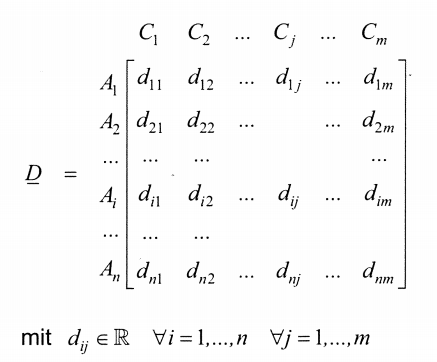
\includegraphics[scale = 0.7]{img/TOPSIS.png}
	\quelle{\cite{Peters.2007}}
	\caption{Matrix mit Alternativen und Kriterien}
	\label{img:topsis}
\end{figure}\\
In den Spalten finden sich jeweils die Bewertungen aller Alternativen in Bezug auf ein Kriterium. Logischerweise steht dann in den Zeilen die Bewertung einer Alternative im Bezug auf alle Kriterien. Für jede Spalte wird dann das Minimum und Maximum gesucht, um dadurch sowohl die obere als auch die untere Grenze zu bestimmen. Dabei ist zu beachten, dass die obere Grenze von Kriterium zu Kriterium unterschiedlich sein kann, da bei manchen Kriterien eine niedrige Bewertung als positiv angesehen wird. Als letzter Schritt werden die euklidischen Distanzen zwischen den Bewertungen der Alternativen und denen der oberen und unteren Grenzen bestimmt. Die Alternative mit der geringsten Gesamtdistanz zur oberen Grenze oder der größten Gesamtdistanz zur unteren ist damit dann die beste Alternative. Außerdem ergibt sich dadurch eine Reihenfolge der Alternativen.\\
Die TOPSIS-Methode ist eine gute Möglichkeit, um schnell eine Reihenfolge aus den vorhandenen Bewertungen zu erhalten. Außerdem benötigt sie wie die Nutzwertanalyse keine zusätzlichen Hilfsmittel und ist mathematisch einfach zu berechnen. Allerdings nutzt sie für die Bewertung der Alternativen eine Methode ähnlich der Nutzwertanalyse, wodurch auch die Vor- und Nachteile dieser Analyse mit einfließen.
\subsection{Auswahl der Methode}
Nach der Vorstellung aller Methoden folgt nun die abschließende Auswahl der im späteren Verlauf der Arbeit eingesetzten Methode. Alle drei Methoden werden verglichen und anhand ihrer Vor- und Nachteile im Kontext der Arbeit bewertet.\\
Ziel dieser Arbeit ist die Evaluation eines \ac{CI}/\ac{CDE}/\ac{CD}-Tools für einen geplanten Service der Abteilung. Dafür muss das Tools bedacht, objektiv und rational ausgewählt werden. Dabei treten sowohl bei der Nutzwertanalyse als auch bei der TOPSIS-Methode die ersten Probleme auf. Die Gewichtungen sowie die Bewertungen werden nur im Kontext des Gesamtproblems getroffen und nicht wie bei der AHP-Analyse durch Paarvergleiche. Dadurch geht die Rationalität zum Teil verloren, da für die Gewichtungen und Bewertungen nicht das vollständige Bild genutzt wird, sondern alles nur in einem bestimmten Kontext gesehen wird. Dadurch entgehen unter Umständen entscheidende Details, die in der AHP-Analyse bedacht werden.\\
Dagegen steht die einfache Anwendung der Nutzwertanalyse und TOPSIS-Methode. Die AHP-Analyse ist deutlich aufwändiger in ihrer Art. Allerdings sind die Bearbeitungszeit und Rahmen dieser Arbeit groß genug, wodurch die Komplexität der Analyse keine große Rolle spielt.\\
Des Weiteren findet bei der TOPSIS-Methode keine Prüfung statt. Weder die Gewichtungen und Bewertungen noch die abschließenden Ergebnisse werden überprüft. Die AHP-Analyse überprüft die Gewichtung ihrer Kriterien auf Konsistenz, und die abschließenden Ergebnisse werden mithilfe einer Sensitivitätsanalyse auf ihre \enquote{Robustheit} geprüft. Mit der Nutzwertanalyse kann man ebenfalls eine Sensitivitätsanalyse durchführen.\\
Abschließend führen alle diese offensichtlichen Nachteile der Nutzwertanalyse und TOPSIS-Methode zum Ausschluss dieser beiden als geeignete Methoden zur Evaluierung der \ac{CI}/\ac{CDE}/\ac{CD}-Tools. Die AHP-Analyse hat erhebliche Vorteile gegenüber den beiden Methoden. Aus diesem Grund werden die \ac{CI}/\ac{CDE}/\ac{CD}-Tools mithilfe der AHP-Analyse evaluiert. Diese wird nun nachfolgend noch einmal genauer erläutert, um eine methodische Basis für die Durchführung der Analyse in Kapitel \ref{pract} zu schaffen.
\section{Analytic Hierarchy Process (AHP-Analyse)}\label{ahp}
Wie kann man rationale Entscheidungen in einer irrationalen Welt treffen? Man kann es nicht. Allerdings ist es möglich, mithilfe von verschiedenen Analysemethoden der Entscheidungstheorie eine möglichst große Näherung an eine rationale Entscheidung zu erreichen. 
\subsection{Einführung}
Eine dieser Methoden ist die \ac{NWA} (siehe \ref{nutz}). Sie ist ein bewährtes Hilfsmittel in Wissenschaft und Wirtschaft, um Entscheidungen zu finden und Möglichkeiten zu bewerten. Indem das Problem fragmentiert wird, kann durch die Methodik der Nutzwertanalyse die vollständige Problematik erfasst werden, oder anders ausgedrückt: \enquote{Das Gesamtproblem, das es zu entscheiden gilt, wird in Teilprobleme zerlegt und diese, wenn erforderlich, wiederum in Teilprobleme}\autocite[S.1]{Kuehnapfel.2014}. Alle Facetten des Problems werden betrachtet und nicht vereinfacht oder abstrahiert. Somit umgeht man die menschliche Natur, die aufgrund einer möglichen Zeitersparnis ein komplexes Problem immer vereinfachen will. Das Vereinfachen führt allerdings zu einer erhöhten Fehlerquote und zum sofortigen Ausschluss von unkonventionellen Möglichkeiten aufgrund der Tendenz des Menschen zu Konstanz und Bewahrung\autocite[Vgl.][S.1]{Kuehnapfel.2014}. Im Gegensatz dazu gewährleistet die Nutzwertanalyse Objektivität und Chancengleichheit unter den verschiedenen Alternativen.\newline
Die Rationalität der Methodik ergibt sich aus der Vorgehensweise bei der Bearbeitung einer Fragestellung. Die einzelnen Fragmente (Kriterien) der Fragestellung werden einzeln bewertet und entsprechend ihrer Relevanz für das Gesamtproblem gewichtet.\autocite[Vgl.][S.10]{Kuehnapfel.2014} An der Auswahl der Kriterien und deren Gewichtung sollten möglichst viele Stackeholder beteiligt sein, um die Einflussnahme einzelner Meinungen zu unterbinden.\\
\\
In den 1970er Jahren hat Thomas L. Saaty das Konzept der \ac{NWA} weiterentwickelt. Der \ac{AHP} ist wie die \ac{NWA} ein grundlegender Ansatz zur Entscheidungsfindung und wurde entworfen, um sowohl rationale als auch intuitive Entscheidungen in die Auswahl von zuvor selektierten Alternativen einzubeziehen.\autocite[Vgl.][S.1]{Saaty.2012} Er heißt Analytischer Hierarchie Prozess, weil er sowohl analytisch, hierarchisch als auch prozessorientiert arbeitet.\autocite[Vgl.][]{TUM.2015}
\begin{itemize}
	\item\texttt{analytisch:} Die Entscheidungsunterstützung erfolgt mathematisch und mittels Logik
	\item\texttt{hierarchisch:} \enquote{Bei Nutzung des AHP sind die für die Erfüllung der Zielstellung genutzten Entscheidungskriterien einer hierarchischen Struktur unterworfen.}\autocite[S.314]{Hausladen.2016} 
	\item\texttt{prozessorientiert:} Die Entscheidungsunterstützung erfolgt immer nach demselben Prozess
\end{itemize}
Während des Prozesses werden einfache paarweise Vergleiche durchgeführt. Die Ergebnisse dieser Vergleiche werden dann genutzt, um eine Reihenfolge der Alternativen zu erstellen.\autocite[Vgl.][S.1]{Saaty.2012}
\subsection{Ablauf des AHP}
Die einfachste Form, ein Entscheidungsproblem in einer AHP-Analyse darzustellen, ist die innerhalb einer Hierarchie mit drei Ebenen.(Abbildung \ref{img:hier})
\begin{figure}[h!]
	\centering
	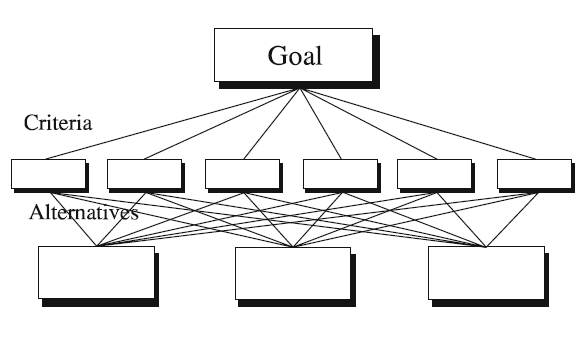
\includegraphics[scale = 0.8]{img/Hierarchie.png}
	\quelle{\cite[S.3]{Saaty.2012}}
	\caption{three level hierarchie}
	\label{img:hier}
\end{figure}
Das Grundproblem wird immer weiter granuliert. Auf der untersten Ebene finden sich die Alternativen, welche mithilfe der Kriterien auf Ebene 2 evaluiert werden. Diese Erkenntnisse werden dann genutzt, um das Ziel der Entscheidung auf der obersten Ebene zu bestimmen.\autocite[Vgl.][S.2]{Saaty.2012}
Damit hat man auch gleich den Startpunkt einer AHP-Analyse bestimmt. 
\subsubsection{Aufstellen des Entscheidungsmodells}
Die Analyse beginnt wie oben bereits beschrieben mit dem Aufstellen des hierarchischen Entscheidungsmodells. Aus dem Entscheidungsproblem wird ein Ziel definiert, welchem eine endliche Anzahl von Alternativen zugeordnet wird $X=\{x_{1}, ..., x_{n}\}$\autocite[Vgl.][S.3]{Brunelli.2015}.
Des Weiteren werden die Kriterien auf deren Basis die Alternativen verglichen werden aus dem Ziel abgeleitet. Sollte die Kriterienanzahl zu groß sein bietet es sich an, diese in Subkriterien aufzuteilen. Dadurch erhält man eine weitere Ebene innerhalb der Hierarchie. Am Ende dieser Phase der AHP-Analyse sollte eine Struktur ähnlich zu Abbildung \ref{img:hier} vorhanden sein. Mit dieser fertig erstellten Hierarchie erhält man eine bessere Übersicht über die Entscheidung, die gefällt wird, die Kriterien, die genutzt werden und die Alternativen, die zur Verfügung stehen.\autocite[Vgl.][S.9]{Mu.2018} 
\subsubsection{Gewichtung der Kriterien}
Nicht alle Kriterien werden die gleiche Relevanz haben. Deswegen werden im zweiten Schritt der AHP-Analyse die Kriterien gewichtet.\autocite[Vgl.][S.9]{Mu.2018} Diese Gewichtung erfolgt relativ zueinander. Relativ bezieht sich dabei auf den Umstand, dass für die Priorisierung der einzelnen Kriterien diese im Verhältnis zueinander bestimmt werden. \\
Damit die Gewichtungen vergleichbar sind, besonders, wenn diese in einem Bewertungsgremium getroffen werden, muss es eine zentrale Skala geben. Mithilfe dieser werden dann die entsprechenden Gewichtungen vorgenommen. Am Ende diese Prozesses soll ein Gewichtungsvektor $w=(w_{1}, ..., w_{n})$ mit einem $w_i$ für jedes $x_i$ aus $X=\{x_{1}, ..., x_{n}\}$ entstehen\autocite[Vgl.][S.4]{Brunelli.2015}.
\begin{figure}[h!]
	\centering
	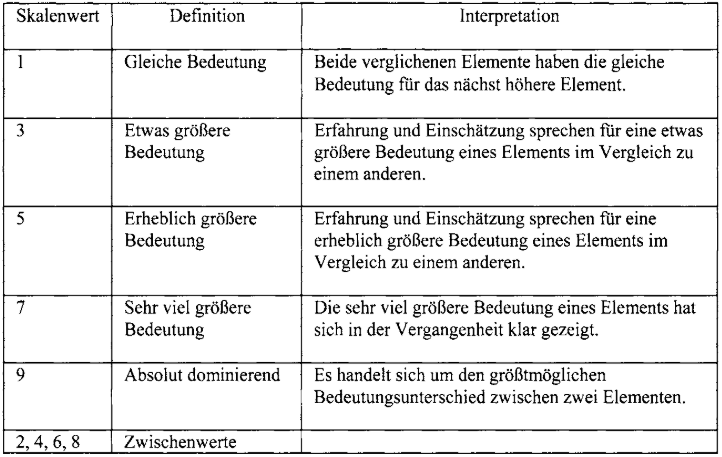
\includegraphics[scale = 0.8]{img/Skala.png}
	\quelle{\cite[S.105]{Fink.2006}}
	\caption{Saaty-Skala}
	\label{img:scale}
\end{figure}\\
Die Schwierigkeit dabei ist die Auswahl der richtigen/passenden Skala. In seinem 1977 veröffentlichen Artikel\autocite{Saaty.1977} vergleicht Saaty verschiedene Skalen miteinander und kommt dabei zu dem Schluss, dass die Skala von 1-9 (Abbildung \ref{img:scale}) die passendste im Hinblick auf die Anwendung mit der AHP-Analyse ist. \\
Mithilfe dieser Skala werden nun die paarweise Vergleiche durchgeführt. Jede Kategorie wird mit jeder anderen einzeln verglichen und mithilfe der Skala bewertet.\autocite[Vgl.][S.106]{Fink.2006}  
\[\begin{array}{rcl}
\centering
x_1 &\leftrightarrow &x_2 \\
x_1 &\leftrightarrow &x_3 \\
x_2 &\leftrightarrow &x_3 \\
\vdots &                &\vdots
\end{array}\]
Am Ende dieses Prozesses sollte eine Matrix ähnlich zu \ref{matrix} entstanden sein.
\begin{table}[h!]
	\ra{1.5}
	\centering
	\[X\quad = \quad\begin{tabular}{l|llll}
	& $x_1$ & $x_2$ &  $x_3$  \\ \hline
	$x_1$ &   1   &   5   &   2   \\
	$x_2$	&$\frac{1}{5}$&   1   &$\frac{1}{3}$     \\
	$x_3$	&$\frac{1}{2}$&   3   &   1         
	\end{tabular} 	  
	\quad bzw. \quad
	\left( \begin{array}{rrrr}
	1   &   5   &   2   \\
	\frac{1}{5}&   1   &\frac{1}{3}     \\
	\frac{1}{2}&   3   &   1        
	\end{array}\right) 
	\]
	\caption{Matrix}
	\label{matrix}
\end{table}
In diesem Beispiel lässt sich erkennen, dass $x_1$ erheblich größere Bedeutung hat als $x_2$. Außerdem hat $x_3$ etwas größere Bedeutung als $x_2$.
\subsubsection{Gewichtungsvektoren}
Mit dieser Tabelle lassen sich jetzt aber noch keine Aussagen treffen. Deswegen werden in diesem Arbeitsschritt die Gewichtungsvektoren $w=(w_{1}, ..., w_{n})$ berechnet.\\
Hierfür gibt es zwei Methoden: das Näherungsverfahren und die Eigenvektormethode. Die Eigenvektormethode kann dabei als theoretischer Grundbaustein der AHP-Analyse angesehen werden.\autocite[Vgl.][S.106]{Fink.2006} Für die nachfolgende Erklärung wird allerdings das Näherungsverfahren beschrieben. Dieses führt\enquote{im Falle vollkommen konsistenter Urteile ebenfalls zu exakten Ergebnissen}\autocite[S.106]{Fink.2006}.
\begin{figure}[h!]
	\centering
	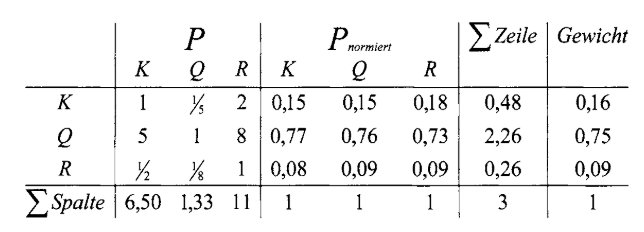
\includegraphics[scale = 0.9]{img/Tabelle.png}
	\quelle{\cite[S.107]{Fink.2006}}
	\caption{Paarvergleichsmatrix}
	\label{img:table}
\end{figure}
Die Berechnung beginnt mit der Normalisierung der Matrix aus dem vorangegangenen Arbeitsschritt. Dafür werden die Spalten zuerst aufsummiert. Danach teilt man jede einzelne Zelle durch die Summe ihrer Spalte. Sobald dies erledigt ist, erhält man das $P_{normiert}$ aus Abbildung \ref{img:table}. Für die abschließenden Gewichtungen müssen jetzt nur noch die Summen der Spalten gebildet werden und durch die Anzahl der Kriterien $n$ geteilt werden. In dem Beispiel \ref{img:table} ergibt sich daraus folgende Reihenfolge für die Kriterien: $Q > K > R$. \\
Hierbei handelt es sich um sogenannte lokale Prioritäten. Saaty teilt die errechneten Prioritäten in lokal und global ein.\autocite[Vgl.][S.16]{Saaty.2012} Dies bezieht sich auf die Gültigkeit der Gewichtungen innerhalb der Hierarchie. Lokale Prioritäten sind nur in ihrer Ebene gültig. Globale Prioritäten gelten für die gesamte Hierarchie. Aus den lokalen Prioritäten lassen sich aber einfach globale berechnen. Sie werden einfach mit den nächsthöheren Ebenen multipliziert $w_n * w_{n-1}$\autocite[Vgl.][S.107]{Fink.2006}. 
\subsubsection{Konsistenz}
Wenn die Gewichtungen getroffen sind, müssen sie auf ihre Konsistenz geprüft werden.\autocite[Vgl.][S.13]{Mu.2018} Sowohl ordinale Transitivität als auch kardinale Konsistenz müssen im Rahmen dessen liegen, was Saaty beschrieben hat.\autocite[Vgl.][S.107]{Fink.2006} Die ordinale Transitivität ergibt sich aus der reinen Logik. Wenn $A > B$ und $B > C$ dann muss auch $A > C$ gelten.\autocite[Vgl.][S.108]{Fink.2006} Die kardinale Konsistenz gibt des Weiteren an, ob die Gewichtungen konsistent sind. \enquote{Ist A zwei Mal besser als B und B drei Mal besser als C, so ist kardinale Konsistenz nur dann gegeben, wenn A sechs Mal besser als C ist.}\autocite[S.107]{Fink.2006} Wenn allerdings Zwischenwerte wie 4, 5 oder 7 zugewiesen werden, kann es zu Inkonsistenzen kommen. In bestimmten Maßen ist dies erlaubt. Sie dürfen nur eine Grenze nicht überschreiten.\autocite[Vgl.][S.13]{Mu.2018} Diese ist mit $CR<=0.10$ festgesetzt. CR bedeutet \enquote{Consistency Ratio} und setzt sich wie folgt zusammen:\autocite[Vgl.][S.13]{Mu.2018}\\
\[CR=\frac{\mbox{\ac{CIx}}}{\mbox{\ac{RI}}}\]\\
\\
\ac{CIx} beschreibt den Consistency Index der zuvor erstellten Matrix. Dieser errechnet sich indem man die Spalten der Ausgangsmatrix \ref{matrix} mit den errechneten Gewichtungen aus \ref{img:table} multipliziert (Siehe Abbildung \ref{img:crit}).
\begin{figure}[h!]
	\centering
	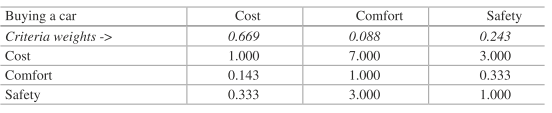
\includegraphics[scale = 1]{img/Kriterien.png}
	\quelle{\cite[S.12]{Mu.2018}}
	\caption{Prioritäten als Faktoren}
	\label{img:crit}
\end{figure}
Danach werden wieder die Summen der Spalten gebildet und durch die jeweiligen Gewichtungen geteilt. Die Ergebnisse werden aufsummiert und durch die Anzahl der Kriterien $n$ geteilt, um den Durchschnitt zu errechnen (Siehe Abbildung \ref{img:lambda}).
\begin{figure}[h!]
	\centering
	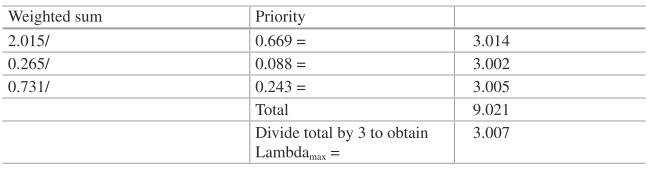
\includegraphics[scale = 0.9]{img/Lambda.png}
	\quelle{\cite[S.14]{Mu.2018}}
	\caption{Berechnung von $\lambda_{max}$}
	\label{img:lambda}
\end{figure} \\
Mit $\lambda_{max}$ lässt sich nun der \ac{CIx} von unserer Matrix berechnen. 
Denn der \ac{CIx} lässt sich wie folgt berechnen:\autocite[Vgl.][S.14]{Mu.2018}
\[CI=\frac{(\lambda_{max}-n)}{(n-1)}\quad \mbox{bzw. für unser Beispiel}\quad CI=\frac{(3.007-3)}{(3-1)}=0.004\]
Damit wir jetzt die \ac{CR} berechnen können, fehlt uns nur noch der \ac{RI}. Hierbei handelt es sich um den \ac{CIx} einer zufällig gefüllten Matrix, welche der Theorie nach sehr inkonsistent sein muss. Saaty stellt praktischerweise schon den durchschnittlichen \ac{CIx} von 500 zufällig gefüllten Matrizen zur Verfügung (Siehe Abbildung \ref{img:ri}).\\
\begin{figure}[h!]
	\centering
	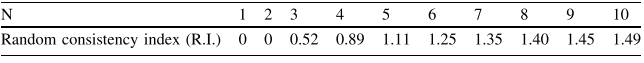
\includegraphics[scale = 0.9]{img/RI.png}
	\quelle{\cite[S.9]{Saaty.2012}}
	\caption{Durchschnittlicher RI}
	\label{img:ri}
\end{figure}\\
Diese sind nach $n$ geordnet und müssen jetzt nur noch in unsere Formel $CR=\frac{\mbox{\ac{CIx}}}{\mbox{\ac{RI}}}$ eingesetzt werden.
\[CR=\frac{\mbox{\ac{CIx}}}{\mbox{\ac{RI}}}=\frac{0.004}{0.52}=0.008\]
Es zeigt sich das $0.008<0.10$. Somit ist die kardinale Konsistenz gegeben, und es kann fortgefahren werden. Sollte dies nicht gegeben sein, muss die Matrix noch einmal überarbeitet werden, um die inkonsistente Stellen zu eliminieren.\autocite[Vgl.][S.108]{Fink.2006}
\subsubsection{Gewichtung der Alternativen}
Nach der Gewichtung der Kriterien werden in diesem Arbeitsschritt die Gewichtungen für die Alternativen berechnet. Die Alternativen werden wie die Kriterien vorher paarweise verglichen, allerdings immer im Hinblick auf ein Kriterium. Hat man also zum Beispiel 3 Kriterien, werden die Alternativen 3 mal im Hinblick auf die Kriterien verglichen. Am Ende entstehen dann 3 Matrizen. 
\begin{figure}[h!]
	\centering
	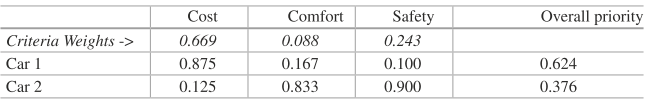
\includegraphics[scale = 0.9]{img/All.png}
	\quelle{\cite[S.19]{Mu.2018}}
	\caption{Modellsynthese}
	\label{img:all}
\end{figure}
Diese werden zusammengefasst und die einzelnen Spalten mit den jeweiligen Prioritäten der Kriterien multipliziert\autocite[Vgl.][S.19]{Mu.2018} (siehe Abbildung \ref{img:all}). Abschließend werden die Summen der Zeilen gebildet. Die Ergebnisse sind dann die globalen Prioritäten und geben die abschließende Reihenfolge der Alternativen an. 
\subsubsection{Sensitivitätsanalyse}
Diese abschließenden Prioritäten sind sehr stark von der Gewichtung der Kriterien beeinflusst.\autocite[Vgl.][S.19]{Mu.2018} Aufgrund dessen wird als letzter Schritt, vor der abschließenden Bewertung, noch eine Sensitivitätsanalyse durchgeführt. Mithilfe dieser wird geprüft, wie \enquote{robust} das Ergebnis der Analyse ist.\autocite[Vgl.][S.20]{Mu.2018} \enquote{Ziel ist es, durch die systematische Verlagerung von Kriteriengewichten Grenzen zu bestimmen, bei denen sich die Reihung von Alternativen umkehrt.}\autocite[S.111]{Fink.2006}\\ 
Getestet wird dies, indem der letzte Schritt der Analyse noch einmal mit veränderten Gewichtungen vorgenommen wird. Was passiert also bei (a) gleichen Gewichtungen, und (b) welche Gewichtung führen zu gleichen Prioritäten?\autocite[Vgl.][S.20]{Mu.2018}\\
Zuerst werden die Gewichtungen aller Kriterien gleichgesetzt. Bei 3 Kategorien würde dies eine jeweilige Gewichtung von $0.333$ bedeuten.\\
Um den \enquote{Break-Even Punkt}\autocite[S.21]{Mu.2018} der Prioritäten zu berechnen kann man sich mithilfe des Ergebnisses aus (a) herantasten. Durch das wiederholte Umstellen der Prioritäten ist es möglich, den \enquote{Break-Even Punkt} zu berechnen. Abschließend werden die Ergebnisse analysiert. \enquote{Führen bereits geringfügige Veränderungen der Kriteriengewichte zu einer [Umkehr der Prioritäten], so ist das ein Hinweis auf ein instabiles Ergebnis. In einem solchen Fall ist es ratsam, den Beurteilungsprozess zu wiederholen bzw. zu überprüfen.}\autocite[S.111]{Fink.2006}
\subsubsection{Finale Entscheidung}
Nachdem alle Schritte vollzogen sind, kann eine finale Entscheidung gefällt werden. Dafür werden die Ergebnisse der Analyse, der Konsistenzanalyse und der Sensitivitätsanalyse einbezogen, um eine aussagekräftige Entscheidung zu treffen, welche Alternative das festgelegte Ziel in Schritt 1 am besten erfüllt.
\chapter{Praktische Umsetzung}\label{pract}
In diesem Teil der Arbeit liegt der Fokus auf der praktischen Anwendung. Es werden die technischen Alternativen vorgestellt und mithilfe der AHP-Analyse verglichen. Doch zuerst folgt eine kurze Einführung in das Projektumfeld.
\section{Projektumfeld}
Diese Bachelorarbeit findet im Umfeld der Atos Information Technology GmbH statt. Das Unternehmen ist die deutsche Tochtergesellschaft des französischen IT-Dienstleisters Atos SE. Die Atos SE ist ein internationaler IT-Dienstleister mit Hauptsitz in Paris. Das Unternehmen deckt unter anderem die Geschäftsfelder Beratungs- und Technologieservices, Systemintegration und Outsourcing-Dienstleistungen ab.\\
Die Abteilung \ac{CAP}, in welcher die Arbeit geschrieben wird, betreibt dabei größtenteils klassische Service Delivery, also die Umsetzung und Lieferung von Kundenanfragen. Mittlerweile gibt es aber auch ein kleines Team von Entwicklern, das sich agil nach DevOps (siehe \ref{devops}) organisiert und proaktiv neue kleinere Projekte angeht. Dabei fokussieren die Entwickler sich besonders auf neue Technologien wie zum Beispiel Angular, NodeJS und auch \ac{CI}/\ac{CDE}/\ac{CD}.\\ 
Dabei merkten sie, dass Continuous Practices einen großen Mehrwert für sie bringen. Jederzeit eine getestete und lauffähige Version ihrer Applikation in der Hand zu haben, hilft ihnen sehr, da sie in Sprints arbeiten. Das heißt, sie haben vorher abgestimmte Arbeitspakete, welche sie dann in einem bestimmten Zeitraum (meistens eine Woche) abarbeiten, um am Ende eine Review mit dem Kunden durchzuführen. Mithilfe der Continuous Practices gibt es immer eine lauffähige Version der Applikation, welche dem Kunden präsentiert werden kann. Außerdem können sie sich vollkommen auf die Entwicklung konzentrieren, da alles andere automatisch im Hintergrund abläuft.\\ 
Diese Vorteile möchte die Abteilung nun auch anderen zur Verfügung stellen. Mit \ac{CI}/\ac{CDE}/\ac{CD} as a Service möchte sie internen so wie externen Kunden die Möglichkeit bieten, einfach in Continuous Practices einzusteigen und damit ihre Entwicklung zu verbessern. Des Weiteren eröffnet sich dadurch eine neue Einnahmequelle für die Abteilung.
%\section{Zieldefinition}
\section{Vorstellung der Alternativen}
Im Folgenden werden die vier zu vergleichenden Alternativen einzeln vorgestellt. Dabei werden sie zum einen allgemein beschrieben, zum anderen wird auf die jeweiligen Besonderheiten eingegangen. Die Auswahl dieser vier Tools wurde im Laufe dieser Arbeit in Zusammenarbeit mit der Abteilung erstellt. Es können nicht alle \ac{CI}/\ac{CDE}/\ac{CD}-Tools am Markt verglichen werden, da dies den Rahmen der Arbeit sprengen würde und die AHP-Analyse eine maximale Anzahl von vier Alternativen vorgibt. Es wurde deswegen bei der Auswahl auf die Vielseitigkeit, und die Größe/Bekanntheit der Tools geachtet.
\subsection{Jenkins CI} Jenkins CI, ehemals Hudson, wurde 2006 von Kohsuke Kawaguchi als Ein-Mann Projekt ins Leben gerufen.\autocite[Vgl.][S.56]{Wiest.2011} Sein Ziel war es langweilige und repetitive Aufgaben während der Entwicklung zu automatisieren. Mittlerweile ist es ein eigenständiges Open-Source Projekt mit MIT-Lizenz und wird von einer großen Community gepflegt. Durch die frühe Umsetzung durch Kawaguchi ist Jenkins das bekannteste und meistgenutzte Tool für \ac{CI}/\ac{CDE}/\ac{CD}.\autocite[Vgl.][]{Jenkins.2019}\\
Jenkins ist ein CI-Server, welcher komplett in Java geschrieben ist und als Java-Webapplikation realisiert wurde. Er muss also in einem Webcontainer laufen.\autocite[Vgl.][S.57]{Wiest.2011} Durch diese Einfachheit lässt sich ein Jenkins Server auf fast allen Systemen installieren. Zum Beispiel in der Cloud, OnPremise oder auch als Container. In seiner Grundstruktur bietet Jenkins nur rudimentäre Grundfunktionen. Die tatsächliche Usability ergibt sich erst durch die große Anzahl an Plugins (1000+),\autocite[Vgl.][]{Jenkins.2019} die von Contributern für Jenkins entwickelt werden. Mithilfe dieser Plugins ermöglicht Jenkins die Unterstützung der meisten Projekte und Plattformen.\\
Durch diese Plugins lassen sich viele Systeme an den Jenkins Server koppeln. Alle gängigen Versionsverwaltungssysteme (siehe \ref{vcs}) wie zum Beispiel Git und Subversion lassen sich dadurch mit Jenkins verknüpfen. Des Weiteren gibt es Plugins für die Anbindung an alle gängigen Datenbanken und sogar an SAP Systeme. Man sieht schnell, dass Jenkins in Sachen Kompatibilität keine Grenzen setzt.\autocite[Vgl.][]{Jenkins.2019}\\
Darüber hinaus bietet Jenkins an, die Last der Pipeline auf verschiedene sogenannte \enquote{Slaves} auszulagern. Diese Slaves sind einfache Systeme, die über den Jenkins Server gesteuert werden und auf seinen Befehl hin Aufgaben ausführen. Dadurch verteilt sich die Last auf das Gesamtsystem, und eine Pipeline kann schneller abgearbeitet werden. Diese Slaves können auch als Docker Container laufen, wodurch die Ressourcen flexibler eingesetzt werden können.\\
Insgesamt ist Jenkins CI ein etabliertes \ac{CI}/\ac{CDE}/\ac{CD}-Tool mit großem Funktionsumfang, das sich vielseitig einsetzten lässt. Durch das erzwungene Eigenhosting und Open Source Quellcode besteht allerdings auch keinerlei Support für etwaige Probleme.
\subsection{Travis CI}
Travis CI ist ein in Deutschland entwickeltes \ac{CI}/\ac{CDE}/\ac{CD}-Tool auf Basis der Programmiersprache Ruby.\autocite[Vgl.][]{Travis.2019} Seit 2013 bietet das Unternehmen Travis CI GmbH \ac{CI}/\ac{CDE}/\ac{CD} als Service an. Dabei haben sie sich auf Github konzentriert. GitHub ist ein Onlinedienst, der Software-Entwicklungsprojekte auf seinen Servern bereitstellt,\autocite[Vgl.][]{GitHub.2019} also einem Onlinehost für das Versionsverwaltungssystem Git (siehe \ref{vcs}). Travis CI lässt sich nur mit Github zusammen betreiben. Dafür sind beide aber auch eng miteinander verzahnt, und die Integration funktioniert ohne Probleme. Ähnlich zu Jenkins CI lässt sich auch bei Travis CI die Last der Pipeline auf mehrere Systeme aufteilen.\\
Travis CI wird in zwei Versionen vom Unternehmen vertrieben\autocite[Vgl.][]{Travis.2019}:
\begin{itemize}
	\item \texttt{As a Service (Cloud)}\\
	Bei dieser Option ist Travis bei der Travis CI GmbH in der Cloud gehostet. Es muss nur eine Datei mit der Travis Konfiguration im Software Repository hinterlegt werden, und Travis übernimmt die weiteren Aufgaben. Am Ende erhält man eine Benachrichtigung mit dem Verlauf der Pipeline. Allerdings wird dies Version nochmal in zwei Optionen aufgeteilt:
	\begin{itemize}
		\item Open Source Projekte\\
		Für Open Source Projekte bietet die Travis CI GmbH ein kostenloses Angebot zur Nutzung ihres Services an. Entwickler von Open Source Projekten haben die Möglichkeit, diesen Service mit Einschränkungen kostenfrei zu nutzten. Die Einschränkungen beziehen sich dabei auf die Leistung, die ihnen zu Verfügung steht. Entwickler können allerdings auch jederzeit auf die kommerzielle und damit nicht mehr kostenfreie Version wechseln, um mehr Leistung zu erhalten.
		\item Kommerzielle Projekte\\
		Für kommerzielle Projekte bietet Travis CI GmbH verschiedene \enquote{Pläne} an für die Nutzung ihres Services. Diese starten bei 69 US-Dollar im Monat und gehen hoch bis zu 489 US-Dollar. Die Unterschiede innerhalb der vier angebotenen Pläne liegt dabei in der Anzahl der gleichzeitig ausführbaren Jobs, also Aufgaben, die parallel ausgeführt werden können.
	\end{itemize}
	\item \texttt{Enterprise Edition (OnPremise)}\\
	Seit 2014 bietet Travis CI GmbH auch die Möglichkeit für Unternehmen, Travis CI OnPremise zu erhalten. Das heißt, dass Unternehmen die Möglichkeit haben, Travis CI lokal auf ihrer Hardware zu hosten. Für viele Unternehmen ist dies sehr wichtig, weil zum Beispiel erhöhte Sicherheitsvorgaben bezüglich der Daten herrschen oder Konfigurationen getätigt werden müssen, um den Anforderungen an das Firmennetz zu genügen. Die Preise für diese OnPremise Lösung starten bei 4000 US-Dollar pro 10 Benutzer pro Jahr und steigen entsprechend linear in Schritten von 10 Benutzern.
\end{itemize}
Travis CI ist eine einfache Möglichkeit, mit \ac{CI}/\ac{CDE}/\ac{CD} zu starten. Durch das Hosting in der Cloud wird dem Nutzer viel Konfigurationsaufwand abgenommen. Außerdem wird ein Kundensupport angeboten, welche bei Problemen eingreifen kann. Allerdings führt die Beschränkung durch Github als einzig unterstütztes Software Repository zu Problemen mit eventuell anderen präferierten Anbietern.
\subsection{Circle CI}
Circle CI wurde 2011 von Paul Biggar und Allen Rohner gegründet. Seitdem hat sich ihr Tool zu einem Leader in ihrer Branche entwickelt.\autocite[Vgl.][]{Forrester.2017} Viele große Kunden nutzen entweder den Service von Circle CI oder betreiben das Tool selbst in ihrer eigenen Umgebung. Zu ihren Kunden zählen Facebook, Spotify und noch mehr bekannte Unternehmen.\autocite[Vgl.][]{Circle.2019} \\
Ihr Angebot ähnelt dabei sehr dem von Travis CI. Sie bieten Circle CI as a Service an und vertreiben dabei verschiedene Konfigurationen mit verschiedenen Leistungsklassen. Die Jobs können dabei entweder in Linux Container laufen oder auf MacOS Systemen. Sie unterscheiden bei den Linux Containern zwischen \enquote{parallelism} und \enquote{concurrency}\autocite[Vgl.][]{Circle.2019}.
\begin{itemize}
	\item \texttt{concurrency}\\
	\enquote{concurrency} bezieht sich dabei auf die Aufteilung von einzelnen Jobs auf verschiedene Container.
	\item \texttt{parallelism}\\
	\enquote{parallelism} bedeutet, dass ein Job auf mehrere Container verteilt wird. Dies führt zu einer enormen Steigerung der Laufzeit dieses Jobs.
\end{itemize}
Bei der Bestellung des Service kann man dabei zwischen diesen beiden Optionen wählen und diese auch kombinieren. Allerdings ist zu beachten, dass bei erhöhtem \enquote{parallelism} nicht mehr viele Jobs gleichzeitig ausgeführt werden können. Die Kosten ändern sich bei Umverteilung allerdings nicht. Er beträgt bei Linux Container 50 US-Dollar pro Container pro Monat. Die MacOS Instanzen starten bei 39 US-Dollar pro Monat und gehen rauf bis 249 US-Dollar für sieben gleichzeitige Jobs.\autocite[Vgl.][]{Circle.2019}\\
Neben Circle CI as a Service wird auch noch eine eigengehostete Alternative angeboten. Hierbei zahlt das Unternehmen pro User pro Monat, anders als bei Travis CI. Der Preis pro Nutzer pro Monat beträgt dabei 35 US-Dollar.\autocite[Vgl.][]{Circle.2019}\\
Circle CI ist insgesamt eine weitere einfache Möglichkeit, um \ac{CI}/\ac{CDE}/\ac{CD} zu betreiben. Circle CI as a Service verspricht einfache Handhabung und die großen Kunden lassen auf Professionalität und Qualität schließen.
\subsection{GitLab CI}
GitLab CI gehört zu dem DevOps Tool GitLab\autocite[Vgl.][]{GitLab.2019}. Dieses wurde 2011 von Dmitri Saparoschez ins Leben gerufen. Bei GitLab handelt es sich um eine Kombination von vielen DevOps Tools. Dazu gehören ein Code Repository, um den Quellcode zu organisieren, ein Kanban Board, um Aufgaben zu tracken und den Fortschritt zu dokumentieren und eben GitLab CI für \ac{CI}/\ac{CDE}/\ac{CD}\autocite[Vgl.][]{GitLab.2019}. Damit hat man alles, was man für ein Softwareprojekt braucht, zentral an einem Ort.\\ 
GitLab CI wurde 2012 mit der Version 3.1.0 von GitLab eingeführt\autocite[Vgl.][]{GitLab.2019}. Seitdem wurde es kontinuierlich weiterentwickelt und verbessert. Die Konfiguration funktioniert ähnlich wie die meisten anderen \ac{CI}/\ac{CDE}/\ac{CD}-Tools. Es wird eine Konfigurationsdatei im Software Repository hinterlegt, welche GitLab CI dann ausliest und abarbeitet.\\
 Die Besonderheit bei GitLab CI ist dabei, dass die Pipeline nicht sofort abgearbeitet werden kann. Es muss erst ein sogenannter \enquote{Runner} definiert werden. Ein Runner kann dabei jegliche Form eines Systems sein, zum Beispiel eine virtuelle Maschine, ein VPS oder auch ein Docker Container. Des Weiteren können auch mehrere Runner zusammen betrieben werden, um die Last zu verteilen. Allerdings bietet GitLab auch Runner auf seiner eigenen Infrastruktur an, sogenannte \enquote{Shared Runner}. Für kostenlose Nutzer stellt GitLab 2000 Minuten Nutzzeit auf diesen Shared Runnern zur Verfügung. Diese können durch monatliche Zahlungen erweitert werden. Es werden drei Pakete für jeweils 4, 19 und 99 US-Dollar pro Monat pro User angeboten. Bei der 99 US-Dollar Variante sind 50000 Minuten auf den Shared Runnern inbegriffen und noch weitere Service Leistungen.\autocite[Vgl.][]{GitLab.2019}\\
Allerdings gibt es auch eine selbstgehostete Variante von GitLab. Hierbei ist die kostenlose Version eine von der Community gepflegten Version von GitLab, GitLab CE (Community Edition).\autocite[Vgl.][]{GitLab.2019} Diese Version ist unter der MIT Lizenz frei verfügbar und kann auf den meisten Linux Distributionen installiert werden. Windows Systeme werden nicht unterstützt. Für weitere Aufpreise von jeweils 4, 19 und 99 US-Dollar pro Monat pro User wird der Funktionsumfang erhöht und ein erweiterter Support angeboten.\autocite[Vgl.][]{GitLab.2019}\\
Insgesamt ist GitLab CI ein ausgereiftes und der Zukunft zugewandtes Tool, welches nicht ohne Grund in der Forrester CI Wave™ auf Platz eins gewählt wurde\autocite[Vgl.][]{Forrester.2017}. Dadurch, dass man immer das gesamte GitLab Toolset einkauft beziehungsweise benutzt, ist man relativ starr in der Hinsicht auf die Nutzung mit anderen Tools. Dafür sind alle Tools innerhalb GitLabs gut miteinander verzahnt und integrieren sich ohne Probleme miteinander.\\ 
\section{Kriterienkatalog}
Im Folgenden werden alle Kriterien einzeln beschrieben und vorgestellt. Dabei werden sie auch voneinander abgegrenzt, um etwaige Überschneidungen in der Definition zu vermeiden. Die Kriterien wurden in einem Meeting am 25.01.2019 mit 4 teilnehmenden Personen erarbeitet. Dabei wurde sich an 4 Prämissen orientiert: 
\begin{itemize}
	\item Geschwindigkeit
	\item Zuverlässigkeit
	\item Kosten
	\item Sicherheit
\end{itemize}
Diese stellen den Anspruch für die Anforderungen an ein \ac{CI}/\ac{CDE}/\ac{CD}-Tool für die Nutzung als Service. Mithilfe dieser Prämissen wurden die nun folgenden Kriterien erstellt. Bei den meisten Kriterien wurden noch Unterkriterien definiert, um das Zielproblem möglichst fein granuliert abzubilden. 
\subsection{Kosten}
Kosten sind essentiell bei der Erstellung eines Services. Kosten sind in jedem Bereich der Wirtschaft ausschlaggebend für Entscheidungen. Sollten die Kosten den Umsatz übersteigen, ist ein Service nicht wirtschaftlich. Aus diesem Grund muss ein \ac{CI}/\ac{CDE}/\ac{CD}-Tool möglichst kostengünstig operierbar sein. Dazu zählt auch die Einschätzung der anfallenden Kosten. Sollten bei einem Tool die Kosten nicht quantifizierbar sein, ist es nicht möglich, passende Preise für den Service anzubieten. Die Kosten gehören dabei zu den messbaren Kriterien. Sie können also anhand von tatsächlichen Werten verglichen werden.
\subsubsection{Monatliche Kosten}
Monatliche Kosten sind monatlich wiederkehrende Kosten. Dazu zählen zum Beispiel Nutzungskosten beziehungsweise Lizenzkosten, Kosten für den Support und auch Serverkosten. Diese gehen aufgrund von Cloud Computing seit Jahren aber schon zurück. Des Weiteren sollten die monatlichen Kosten nach Möglichkeit nicht linear mit der Anzahl der Kunden steigen, da sonst weniger Marge verbucht werden kann.
\subsubsection{Initiale Kosten}
Die initialen Kosten für ein Tools können sich auf verschiedene Weisen zusammensetzten. Dazu können Lizenzkosten und auch das initiale Einrichten der Tools zählen. Wenn der Aufwand bei der Einrichtung des Tools sehr hoch ist, muss ein Mitarbeiter natürlich länger arbeiten, was zu Mehrkosten führt. 
\subsection{Erweiterbarkeit}
Bei der Erweiterbarkeit geht es sowohl um einen erweiterbaren Funktionsumfang als auch um eine erweiterte Anbindung an Systeme von Dritten. Der spätere Service soll vielseitig einsetzbar sein. Dafür muss auch das Tool dementsprechend erweiterbar sein, um die geforderten Funktionalitäten anbieten zu können. Dabei sind allerdings auch schon die gegebenen Funktionalitäten aus der Grundsoftware zu beachten, falls diese die Funktionen schon mitbringen. Ohne gewisse Funktionalitäten kann ein Tool nicht eingesetzt werden.
\subsubsection{Anbindung}
Die Anbindung an andere Systeme ist essentiell für den Einsatz in verschiedenen Projekten. Verschiedene Kunden haben verschiedene Konzepte für ihre Software Architektur. Somit muss auch das \ac{CI}/\ac{CDE}/\ac{CD}-Tool mit diesen verschiedenen Architekturen nutzbar sein. Denn das Tool muss sich nach der Architektur richten und nicht die Architektur nach dem Tool. Am besten werden Standardschnittstellen angeboten, mit denen die meisten Programme umgehen können.
\subsubsection{Art der Software}
Die Art der Software bezieht sich in diesem Fall darauf, ob es sich bei dem Tool um  Open Source oder proprietäre beziehungsweise kommerzielle Software handelt. Dabei haben alle Alternativen ihre Vor- und Nachteile. Bei Open Source Software ist der Quellcode quelloffen zu finden, und alle Teile einer Software können nachvollzogen, beziehungsweise im schlimmsten Fall auch geändert werden. Allerdings gibt es auch keine Person, die im Fall von zum Beispiel Sicherheitslücken oder ähnlichen Fehlern haftbar gemacht werden kann. Proprietäre Software dagegen stellt ihren Quellcode nicht zur Verfügung. Dafür haftet der Hersteller für seine Software und ist immer bemüht, relevante Änderungen schnell in das Programm einzupflegen. Bei Open Source Software kann dies unter Umständen länger dauern.
\subsection{Flexibilität}
Bei der Flexibilität der Tools geht es um die Flexibilität bei der Installation der verschiedenen Tools. Wenn ein Tool auf vielen Betriebssystemen betrieben werden kann, ist es sehr viel flexibler einsetzbar. Das bezieht sich sowohl auf OnPremise Distributionen als auch auf die Cloud. Je vielfältiger ein Tool gehostet werden kann, umso mehr kommt es für die Nutzung infrage. Denn auch hierbei kann der Kunde verschiedene Anforderungen und Systeme bereitstellen. Wenn ein Tool innerhalb eines Containers wie zum Beispiel Docker betrieben werden kann, erhöht dies die Einsatzgebiete schlagartig. Die meisten großen \ac{IaaS}-Anbieter bieten mittlerweile einfache Möglichkeiten, um Container auf ihrer Hardware zu betreiben. Des Weiteren wird so die Möglichkeit geschaffen Software auf Betriebssystemen laufen zu lassen, obwohl diese Software normalerweise nicht mit diesem Betriebssystem kompatibel ist.
\subsection{Performance}
Performance ist ein kritischer Punkt bei der Auswahl eines Tools. Wenn Aufgaben zu lange Laufzeiten haben, können die Entwickler ihre Änderungen nicht mehr regelmäßig bauen und testen. Dies führt zu einer Verlangsamung der gesamten Entwicklung. Aus diesem Grund sollte ein Tool möglichst performant sein und Aufgaben effektiv bearbeiten. Am Besten wird eine Möglichkeit geboten, die Last der Prozesse oder Aufgaben auf mehrere Systeme zu verteilen. Dies kann zu einer enormen Leistungssteigerung führen. 
\subsection{Zuverlässigkeit}
Im Kontext der \ac{CI}/\ac{CDE}/\ac{CD}-Tools bedeutet Zuverlässigkeit ein robustes Tool ohne viele Ausfälle und einem überschaubaren Wartungsaufwand. Durch wenig Downtime der Tools wird die allgemeine Produktivität gesteigert, weil die Entwickler durchgängig bauen und testen können. Aus diesem Grund sollten Fehler in einem Tool schnell gelöst werden können. Außerdem ist es von Vorteil, wenn ein Tool in kurzer Zeit hochgefahren werden kann, beziehungsweise neu gestartet werden kann. Des Weiteren müssen Daten persistent gespeichert werden, ohne dass sie verloren gehen. Auch wenn es keine Produktivdaten sind, halten \ac{CI}/\ac{CDE}/\ac{CD}-Tools trotzdem wichtige Daten über den Verlauf einer Entwicklung.
\subsubsection{Support}
Unter Support ist der eventuell vorhandene Unterstützung des Herstellers beziehungsweise der Entwickler des Tools gemeint, sowohl bei Fragen als auch bei auftretenden Problemen. Dabei geht es sowohl um die Erreichbarkeit des Supports als auch um die Zeit, die gebraucht wird bis ein Problem behoben ist. Des Weiteren wird der Umfang der Dokumentation und Problemlösungsportale betrachtet. Diese können bei bekannten Problemen schnell helfen, um diese zu lösen. Dabei ist es wichtig, dass sie gepflegt werden und regelmäßige Updates stattfinden.
\subsubsection{Erreichbarkeit}
Bei der Erreichbarkeit geht es ähnlich wie oben beschrieben um die Erreichbarkeit der laufenden Systeme. Dafür wird auf die Fehlertoleranz der Systeme geachtet und auf die Wiederherstellungszeiten nach einem Absturz. Nach Möglichkeit sollte ein System immer erreichbar sein. Ansonsten entsteht ein Backlog, der die Entwicklung hemmt. Dieser muss dann erstmal abgearbeitet werden, bevor wieder neue Aufgaben erstellt werden können. Somit sollte ein Tool möglichst wenig Downtime haben, um effektiv arbeiten zu können.
\subsection{Sicherheit}
Die Sicherheit eines Tools ist sehr wichtig für eine Entscheidung. Auch wenn es auf den ersten Blick nicht so aussieht, werden sehr viele vertrauliche und sensitive Daten durch ein \ac{CI}/\ac{CDE}/\ac{CD}-Tool geführt. Darunter fallen zum Beispiel die Zugangsdaten zu den verschiedenen angeschlossenen Systemen. Diese müssen meistens im \ac{CI}/\ac{CDE}/\ac{CD}-Tool hinterlegt werden, damit dieses Zugriff auf die Systeme bekommt. Diese Zugangsdaten müssen sicher hinterlegt werden, damit Unbefugte keine Chance haben, diese Daten auszulesen, weder als unbefugter Nutzer noch als Person von außen. Des Weiteren ist der Quellcode im Zweifelsfall auch schützenswert. Wenn es sich nicht gerade um Open Source Projekte handelt , sind der Quellcode beziehungsweise fertige Programme wichtige Assets der Unternehmen. Sollte dieser Quellcode in fremde Hände gelangen, bedeutet das im Zweifelsfall einen enormen Schaden für das Unternehmen. Es sollte immer auf die Sicherheit eines Systems geachtet werden, und versucht werden es so gut wie möglich abzusichern.
\section{Analyse}
Dieser Abschnitt der Arbeit widmet sich nun der Durchführung der AHP-Analyse. Dabei wird nach dem Vorgehen aus Abschnitt \ref{ahp} gearbeitet. Zuerst wird das Zielsystem mitsamt des Ziels der Analyse den Kriterien und den Alternativen aufgestellt. Dies dient als Ausgangspunkt der Analyse. Danach werden die Gewichtungen der Kriterien ermittelt. Außerdem werden alle Alternativen im Hinblick auf jedes Kriterium bewertet. Am Ende wird beides zusammengeführt, um die abschließende Reihenfolge der Alternativen zu ermitteln. Diese Ergebnisse werden dann noch auf Inkonsistenzen geprüft, und die Empfindlichkeit der Ergebnisse gegenüber Veränderungen der Basiswerte wird überprüft.
\subsection{Aufstellen des Zielsystems}
\begin{figure}[h!]
	\centering
	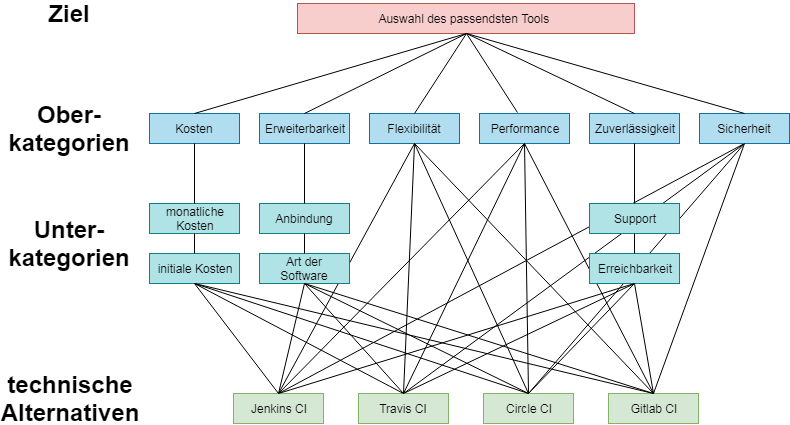
\includegraphics[angle=90, scale = 0.7]{img/ZIEL.png}
	\caption{Zielsystem der Analyse}
	\label{img:ziel}
\end{figure}
In Abbildung \ref{img:ziel} ist das fertige Zielsystem zu sehen. Auf der obersten Ebene findet sich das Ziel, das erreicht werden soll. In der zweiten Ebene werden die Oberkriterien aufgeführt. Die jeweiligen Unterkriterien befinden sich unter ihren Oberkriterien. Auf der untersten Ebene werden die vier Alternativen aufgeführt. Diese sind mit jeweils jedem Kriterium verbunden, da sie alle im Bezug zu jedem einzelnen bewertet werden. Das Zielsystem gibt einen guten Überblick über die gesamte Analyse mit allen eingebrachten Parametern.
\subsection{Gewichtung der Kriterien}
Im folgenden Abschnitt werden nun die Kriterien gewichtet. Dafür wurden die aufgestellten Kriterien aus dem Meeting am 25.01.2019 von allen teilnehmenden Personen bewertet. Da ein Konsens in einer Gruppe immer schwierig ist, gab jede Person ihre eigene Bewertung ab, so dass bei jedem Vergleich 4 Bewertungen vorhanden sind. Aus diesen wurde dann immer der Durchschnitt gebildet. Da dies oft zu einem Ergebnis im Dezimalzahlenbereich führte, wurden die Ergebnisse gerundet. 
\subsubsection{Bewertung der Oberkriterien}
\begin{table}[h!]
	\ra{1.5}
	\centering
	\begin{tabular}{c|cccccc}
		Oberkriterien   & Kosten			 & Erweiterbarkeit & Flexibilität & Performance   \\ 
		\hline
		Kosten          & 1     		      &        6        &       6      &      7      \\
		Erweiterbarkeit &   $\frac{1}{6}$     & 1               &       6      &      3      \\
		Flexibilität    &   $\frac{1}{6}$     &  $\frac{1}{6}$   & 1            &      $\frac{1}{3}$       \\
		Performance     &    $\frac{1}{7}$    &  $\frac{1}{3}$   &        3      & 1           \\
		Zuverlässigkeit &    $\frac{1}{2}$    &          3       &        7      &      3       \\
		Sicherheit      &    1   			  &        6         &        9      &       9             
	\end{tabular}
	\begin{tabular}{c|cc}
		 				&	Zuverlässigkeit & Sicherheit  \\ 
		\hline
		Kosten          &        2        &        1    \\
		Erweiterbarkeit &        $\frac{1}{3}$        &       $\frac{1}{6}$      \\
		Flexibilität    &        $\frac{1}{7}$         &      $\frac{1}{9}$       \\
		Performance     &        $\frac{1}{3}$         &      $\frac{1}{9}$       \\
		Zuverlässigkeit & 1               &      2       \\
		Sicherheit      &        $\frac{1}{2}$       & 1          
	\end{tabular}
	\caption{Gewichtungsmatrix}
	\label{all}
\end{table}
In \ref{all} ist die endgültige Matrix zu sehen. Jedes Kriterium hat eine Bewertung im Vergleich zu allen anderen Kriterien erhalten. Dabei fällt schnell auf, dass einige Kriterien deutlich bessere Bewertungen im Vergleich zu den anderen Kriterien erhalten haben. Zum Beispiel ist deutlich erkennbar, dass Kosten allen Kriterien gegenüber besser bewertet wurde außer Sicherheit. Dasselbe gilt für Sicherheit in gleicher Weise. Allerdings lassen sich mit dieser Matrix noch keine endgültige Aussage über die Gewichtung der einzelnen Kriterien treffen. Zuerst muss die Matrix normalisiert werden, um die Zeilen zu summieren.\\
Vorher werden aber noch die Gewichtungen der Unterkriterien kurz dargestellt.
\subsubsection{Bewertung der Unterkriterien}
\begin{table}[h!]
		\ra{1.5}
		\centering
	\begin{tabular}{c|cc}
		Kosten            & monatliche Kosten & initiale Kosten  \\ 
		\hline
		monatliche Kosten & 1                &          3        \\
		initiale Kosten   &     $\frac{1}{3}$           & 1               
	\end{tabular}
	\caption{Gewichtungsmatrix der Unterkriterien von Kosten}
	\label{cost}
\end{table}
In \ref{cost} ist die Gewichtungsmatrix der Unterkriterien zum Oberkriterium  Kosten zu sehen. Dabei wurden monatliche Kosten mit einer 3 gegenüber den initialen Kosten beurteilt. Die monatlichen Kosten sind damit von \enquote{etwas größerer Bedeutung} (siehe \ref{img:scale}) gegenüber den initialen Kosten. Die monatlichen Kosten sind auf Dauer gesehen der größere Kostenfaktor. Allerdings können hohe initiale Kosten auch abschreckend wirken. Aus diesem Grund wurde die 3 ausgewählt.
\begin{table}[h!]
	\ra{1.5}
	\centering
	\begin{tabular}{c|cc}
		Erweiterbarkeit  & Anbindung & Art der Software  \\ 
		\hline
		Anbindung        & 1         &        5           \\
		Art der Software &    $\frac{1}{5}$       & 1                
	\end{tabular}
	\caption{Gewichtungsmatrix der Unterkriterien von Erweiterbarkeit}
	\label{extend}
\end{table}\\
In \ref{extend} ist die Gewichtungsmatrix der Unterkriterien zum Oberkriterium Erweiterbarkeit zu sehen. Dabei wurde die Anbindung mit einer 5 gegenüber der Art der Software beurteilt. Die Anbindung ist damit von \enquote{erheblich größerer Bedeutung} gegenüber der Art der Software. Es ist wichtiger ein Programm zu erweitern, indem man es an andere Systeme anbindet. Die Möglichkeit den Quellcode anzuschauen und zu verändern, ist dabei weniger wichtig. Deswegen wurde die 5 ausgewählt.
\begin{table}[h!]
	\ra{1.5}
	\centering
	\begin{tabular}{c|cc}
		Zuverlässigkeit & Support & Erreichbarkeit  \\ 
		\hline
		Support         & 1       &        $\frac{1}{4}$         \\
		Erreichbarkeit  &    4     & 1              
	\end{tabular}
	\caption{Gewichtungsmatrix der Unterkriterien von Zuverlässigkeit}
	\label{avail}
\end{table}\\
In \ref{avail} ist die Gewichtungsmatrix der Unterkriterien zum Oberkriterium Zuverlässigkeit zu sehen. Dabei wurde die Erreichbarkeit mit einer 4 gegenüber dem Support beurteilt. Die Erreichbarkeit ist damit in einem Zwischenschritt zwischen \enquote{etwas größerer Bedeutung} und \enquote{erheblich größerer Bedeutung} gegenüber dem Support. Es ist somit wichtiger, ein erreichbares System zu haben anstatt eines erreichbaren Supports.
\subsubsection{Gewichtungsmatrizen}
\begin{table}[h!]
	\ra{1.5}
	\centering
	\begin{tabular}{c|cccccc}
		Oberkriterien   & Kosten			 & Erweiterbarkeit & Flexibilität & Performance   \\ 
		\hline
		Kosten          & 1     		      &        6        &       6      &      7      \\
		Erweiterbarkeit &   $\frac{1}{6}$     & 1               &       6      &      3      \\
		Flexibilität    &   $\frac{1}{6}$     &  $\frac{1}{6}$   & 1            &      $\frac{1}{3}$       \\
		Performance     &    $\frac{1}{7}$    &  $\frac{1}{3}$   &        3      & 1           \\
		Zuverlässigkeit &    $\frac{1}{2}$    &          3       &        7      &      3       \\
		Sicherheit      &    1   			  &        6         &        9      &       9       \\
		\hline
		Summe $\sum$    &  		2,967			&		13,5		&		32		&	23,33
	\end{tabular}
	\begin{tabular}{c|cc}
		&	Zuverlässigkeit & Sicherheit  \\ 
		\hline
		Kosten          &        2        &        1    \\
		Erweiterbarkeit &        $\frac{1}{3}$        &       $\frac{1}{6}$      \\
		Flexibilität    &        $\frac{1}{7}$         &      $\frac{1}{9}$       \\
		Performance     &        $\frac{1}{3}$         &      $\frac{1}{9}$       \\
		Zuverlässigkeit & 1               &      2       \\
		Sicherheit      &        $\frac{1}{2}$       & 1       \\
				\hline
		Summe $\sum$    &  		4,309			&   4,38
	\end{tabular}
	\caption{Gewichtungsmatrix mit Spaltensummen}
	\label{allp}
\end{table}
Nachdem alle Ober und Unterkriterien bewertet wurden, können nun die jeweiligem Gewichtungsmatrizen aufgestellt werden. Dafür werden die Summen der Spalten gebildet, um damit die Matrix zu normalisieren (siehe Tabelle \ref{allp}). Dafür wurde das Tabellenkalkulationstool Excel verwendet.
\begin{table}[h!]
	\ra{1.5}
	\centering
	\begin{tabular}{c|cccccc}
		Oberkriterien   & Kosten			 & Erweiterbarkeit & Flexibilität & Performance   \\ 
		\hline
		Kosten          & 0,33    	  & 0,44    &       0,18  &      0,3      \\
		Erweiterbarkeit &   0,05     & 0,07    &       0,18  &      0,12      \\
		Flexibilität    &   0,05     &  0,01   & 0,03            &      0,01       \\
		Performance     &    0,04    &  0,02   &        0,09      & 0,04           \\
		Zuverlässigkeit &    0,16    & 0,22    &        0,21      &      0,12       \\
		Sicherheit      &    0,33    &  0,44   &        0,28      &       0,38       \\
		\hline
		Summe $\sum$    &  	1			&	1		&		1		&	1
	\end{tabular}
	\begin{tabular}{c|cc|c|c}
		&	Zuverlässigkeit & Sicherheit &$\sum$ Zeile& Gewicht \\ 
		\hline
		Kosten          &        0,46        &        0,22   &1,91 &0,318\\
		Erweiterbarkeit &        0,07        &       0,03   &  0,52& 0,086\\
		Flexibilität    &        0,03         &      0,02    & 0,15 & 0,025\\
		Performance     &        0,07         &      0,02    &  0,28& 0,046\\
		Zuverlässigkeit & 0,23               &      0,45     &  1,38&0,23\\
		Sicherheit      &        0,11       & 0,22    &  1,76& 0,293\\
		\hline
		Summe $\sum$    &  		1			&   1 &6 &1
	\end{tabular}
	\caption{Normierte Matrize}
	\label{allp2}
\end{table}\\
Nachdem alle Summen gebildet sind und in die unterste Zeile eingetragen wurden, können die Spalten normalisiert werden. Das heißt, für jedes Element $x_{n,m}$ aus der Matrix \ref{allp} wird das Folgende berechnet:
\[x_{n,m}(neu)=\frac{x_{n,m}}{\sum(n)}\]
$x_{n,m}$ steht dabei für ein Element aus der Matrix \ref{allp}. Das Element $x_{2,4}$ wäre in diesem Fall der Wert $\frac{1}{3}$ in der zweiten Spalte und vierten Zeile der Matrix. Jedes Element $x_{n,m}$ wird dann durch die Summe seiner Spalten $\sum(n)$ geteilt. Dadurch erhält man $x_{n,m}(neu)$ dessen Wert dann in eine neue Matrize eingetragen wird. Alle Spalten erhalten dadurch ein einheitliches Maß. Dies erleichtert die folgenden Analyseschritte erheblich.

Am Ende dieses Schrittes steht die vollständig gefüllte Matrize \ref{allp2}. Dort sind alle Spalten gefüllt bis auf $\sum Zeile$ und die Gewichtungen. Diese werden als nächster Arbeitsschritt berechnet. Dafür werden zuerst die Summen der einzelnen Zeilen gebildet und in die Spalte $\sum Zeile$ eingetragen. Damit erhält man die abschließenden Gewichtungen. Allerdings sind diese alle mit der Anzahl der Kriterien multipliziert. Deswegen wird als letzter Schritt jedes Element der Spalte $\sum Zeile$ durch die Anzahl der Kriterien geteilt. Dadurch ergeben sich die fertigen Gewichtungen in der letzten Spalte. Nach absteigender Reihenfolge ergeben sich folgende Gewichtungen:
\begin{itemize}
	\item \textbf{1:} Kosten \enspace\dotfill\enspace 0,318\enspace\enspace\enspace
	\item \textbf{2:} Sicherheit \enspace\dotfill\enspace 0,293\enspace\enspace\enspace
	\item \textbf{3:} Zuverlässigkeit \enspace\dotfill\enspace 0,23\enspace\enspace\enspace
	\item \textbf{4:} Erweiterbarkeit \enspace\dotfill\enspace 0,086\enspace\enspace\enspace
	\item \textbf{5:} Performance \enspace\dotfill\enspace 0,046\enspace\enspace\enspace
	\item \textbf{6:} Flexibilität \enspace\dotfill\enspace 0,025\enspace\enspace\enspace
\end{itemize}
Kosten und Sicherheit werden dabei am stärksten gewichtet. Mit jeweils knapp 0,3 machen sie zusammen fast zwei Drittel der Gewichtungen aus. Es zeigt sich also, dass diese beiden Kriterien im Vergleich zu allen anderen Kriterien den Teilnehmern des Meetings am wichtigsten sind. Bevor diese allerdings wirklich genutzt werden können, muss noch ein Konsistenztest gemacht werden. Vorher werden aber noch die Gewichtungen der Unterkriterien ausgerechnet. 
\begin{table}[h!]
	\ra{1.5}
	\centering
	\begin{tabular}{c|cc|cc|c|c}
		Kosten            & mon. K. & i. K & mon. K.& i. K.&$\sum Zeile$& Gewicht\\ 
		\hline
		mon. Kosten & 1                &          3    &  0,75  &0,75 & 1,5&0,75\\
		initiale Kosten   &     $\frac{1}{3}$           & 1   &0,25  & 0,25& 0,5&0,25\\
		\hline
		Summe $\sum$    &  		1,33			&   4        & 1&1 &2 &1
	\end{tabular}
	\caption{Gewichtungen der Unterkriterien von Kosten}
	\label{cost2}
\end{table}\\
In \ref{cost2} ist die komplette Berechnung der Gewichtungen der Unterkriterien zu Kosten zu sehen. Am Ende werden die monatlichen Kosten mit 0,75 und die initialen Kosten mit 0,25 bewertet. Das deckt sich mit der anfänglichen Bewertung von 3 gegenüber den initialen Kosten. Am Ende haben monatliche Kosten eine drei mal so hohe Gewichtung wie die initialen Kosten. Allerdings gelten diese Gewichtungen nur auf ihrer Ebene. Es handelt sich um lokale Prioritäten. Um die globalen Prioritäten zu berechnen, müssen diese Gewichtungen jetzt mit denen ihres Oberkriteriums verrechnet werden. Es gilt:
\[Globale\; Priorität = Priorität_{n}*Priorität_{n-1}\]
Somit ergibt sich für die monatlichen Kosten eine globale Priorität von:
\[0,75\; (Gewichtung\; lokal) * 0,318\; (Gewichtung\; Kosten) =0,238\]
Diese Gewichtung kann nun später genutzt werden, um die Bewertungen der Alternativen durchzuführen.
\begin{table}[h!]
	\ra{1.5}
	\centering
	\begin{tabular}{c|cc|cc|c|c}
		Zuverlässigkeit           & Support & Erreichb. & Support& Erreichb.&$\sum Zeile$& Gewicht\\ 
		\hline
		Support & 1                &           $\frac{1}{4}$   &  0,2  &0,2 & 0,4&0,2\\
	Erreichbarkeit   &         4      & 1   &0,8  & 0,8& 1,6&0,8\\
		\hline
		Summe $\sum$    &  		5			&   1,25        & 1&1 &2 &1
	\end{tabular}
	\caption{Gewichtungen der Unterkriterien von Zuverlässigkeit}
	\label{avail2}
\end{table}\\
In \ref{avail2} und \ref{extend2} finden sich die weiteren Berechnungen der restlichen Unterkriterien von Zuverlässigkeit und Erweiterbarkeit. Bei den Unterkriterien von Zuverlässigkeit ergeben sich für Support und Erreichbarkeit globale Prioritäten von 0,046 und 0,184.\\ \\
Für Anbindung und Art der Software ergeben sich globale Prioritäten von 0,071 und 0,015. 
\begin{table}[h!]
	\ra{1.5}
	\centering
	\begin{tabular}{c|cc|cc|c|c}
		Erweiterbarkeit           & Anbind. & Art d. S. & Anbind.& Art d. S.&$\sum Zeile$& Gewicht\\ 
		\hline
		Anbindung & 1                &          5    &  0,83  &0,83 & 1,66&0,83\\
		Art der Software   &     $\frac{1}{5}$           & 0,17   &0,17  & 0,34& 0,5&0,17\\
		\hline
		Summe $\sum$    &  		1,2			&   6        & 1&1 &2 &1
	\end{tabular}
	\caption{Gewichtungen der Unterkriterien von Erweiterbarkeit}
	\label{extend2}
\end{table}\\
Die Konsistenz aller Unterkriterien ist einfach zu überprüfen und stimmt auch überall. Weder bei Kosten, Zuverlässigkeit noch bei Erweiterbarkeit sind Inkonsistenzen vorhanden. Bei 2 Kriterien pro Oberkriterium ist dies allerdings auch sehr unwahrscheinlich. Bei den Oberkriterien kann dies aufgrund der Anzahl der Kriterien schon eher passieren. Aus diesem Grund wird nun eine Konsistenzprüfung der Oberkriterien durchgeführt.\newpage
Vorher wird aber noch eine Übersicht aller globaler Prioritäten gegeben:  
\begin{itemize}
	\item \textbf{1:} Kosten \enspace\dotfill\enspace 0,318\enspace\enspace\enspace
	\begin{itemize}
		\item \textbf{1:} Monatliche Kosten \enspace\dotfill\enspace 0,238\enspace\enspace\enspace
		\item \textbf{2:} Initiale Kosten \enspace\dotfill\enspace 0,08\enspace\enspace\enspace
	\end{itemize}
	\item \textbf{2:} Sicherheit \enspace\dotfill\enspace 0,293\enspace\enspace\enspace
	\item \textbf{3:} Zuverlässigkeit \enspace\dotfill\enspace 0,23\enspace\enspace\enspace
	\begin{itemize}
		\item \textbf{1:} Erreichbarkeit \enspace\dotfill\enspace 0,184\enspace\enspace\enspace
		\item \textbf{2:} Support \enspace\dotfill\enspace 0,046\enspace\enspace\enspace
	\end{itemize}
	\item \textbf{4:} Erweiterbarkeit \enspace\dotfill\enspace 0,086\enspace\enspace\enspace
	\begin{itemize}
		\item \textbf{1:} Anbindung \enspace\dotfill\enspace 0,071\enspace\enspace\enspace
		\item \textbf{2:} Art der Software \enspace\dotfill\enspace 0,015\enspace\enspace\enspace
	\end{itemize}
	\item \textbf{5:} Performance \enspace\dotfill\enspace 0,046\enspace\enspace\enspace
	\item \textbf{6:} Flexibilität \enspace\dotfill\enspace 0,025\enspace\enspace\enspace
\end{itemize}
\newpage
\subsubsection{Konsistenz}
Damit die Konsistenz geprüft werden kann, müssen zuerst die gewichteten Summen errechnet werden. Dafür werden die Anfangsbewertungen der Kriterien mit den berechneten Gewichtungen aus \ref{allp2} verrechnet. Jedes Element wird mit der Gewichtung des Kriteriums seiner Spalte multipliziert. In Tabelle \ref{all3} ist die Aufstellung der Prioritäten als Faktoren zu sehen.
\begin{table}[h!]
	\ra{1.5}
	\centering
	\begin{tabular}{c|cccccc}
		Oberkriterien   & Kosten			 & Erweiterbarkeit & Flexibilität & Performance   \\ 
		\hline
\textit{Kriteriengewichtung}          & 0,381     		      &        0,086        &       0,025      &      0,046      \\
		Kosten          & 1     		      &        6        &       6      &      7      \\
		Erweiterbarkeit &   $\frac{1}{6}$     & 1               &       6      &      3      \\
		Flexibilität    &   $\frac{1}{6}$     &  $\frac{1}{6}$   & 1            &      $\frac{1}{3}$       \\
		Performance     &    $\frac{1}{7}$    &  $\frac{1}{3}$   &        3      & 1           \\
		Zuverlässigkeit &    $\frac{1}{2}$    &          3       &        7      &      3       \\
		Sicherheit      &    1   			  &        6         &        9      &       9             
	\end{tabular}
	\begin{tabular}{c|cc}
		&	Zuverlässigkeit & Sicherheit  \\ 
		\hline
		\textit{Kriteriengewichtung}         &        0,23        &        0,293    \\
		Kosten          &        2        &        1    \\
		Erweiterbarkeit &        $\frac{1}{3}$        &       $\frac{1}{6}$      \\
		Flexibilität    &        $\frac{1}{7}$         &      $\frac{1}{9}$       \\
		Performance     &        $\frac{1}{3}$         &      $\frac{1}{9}$       \\
		Zuverlässigkeit & 1               &      2       \\
		Sicherheit      &        $\frac{1}{2}$       & 1          
	\end{tabular}
	\caption{Prioritäten als Faktoren}
	\label{all3}
\end{table}\\
Die Prioritäten werden mit jedem Element ihrer Spalte multipliziert, um die gewichteten Summen bilden zu können. Diese lassen sich durch das Summieren der Zeilenwerte berechnen. Dabei ergeben sich Summen, die in der Reihenfolge zu der Reihenfolge der Gewichtungen der Kriterien passen. In der Zeile \enquote{Kosten} ergibt sich die größte Summe, gefolgt von Sicherheit und Zuverlässigkeit (siehe Tabelle \ref{all4}). Die summierten Zeilenwerte werden benötigt, um $\lambda_{max}$ zu berechnen.\\ \\
\begin{table}[h!]
	\ra{1.5}
	\centering
	\begin{tabular}{c|cccccc}
		Oberkriterien   & Kosten			 & Erweiterbarkeit & Flexibilität & Performance   \\ 
		\hline
\textit{Kriteriengewichtung}& 0,381   &   0,086    &       0,025      &      0,046      \\
\hline
		Kosten          & 0,381    	  &   0,516    &       0,15      &      0,322     \\
		Erweiterbarkeit &   0,063     & 0,086      &       0,15      &      0,138      \\
		Flexibilität    &   0,063     &  0,014   & 0,025           &      0,015      \\		
		Performance     &    0,054    &  0,028   &        0,075      & 0,046          \\		
		Zuverlässigkeit &   0,19    &    0,258    &        0,175     &      0,138       \\		
		Sicherheit      &    0,381   &   0,516     &        0,225     &       0,414            
	\end{tabular}
	\begin{tabular}{c|cc|c}
		&	Zuverlässigkeit & Sicherheit  &gew. Summen\\ 
		\hline
		\textit{Kriteriengewichtung}         &        0,23        &        0,293  &  \\
		\hline
		Kosten          &        0,46        &        0,293 &  2,122 \\
		Erweiterbarkeit &        0,076       &       0,048  & 0,561 \\
		Flexibilität    &       0,023        &     0,032   &   0,172\\		
		Performance     &       0,076        &      0,032   & 0,311  \\		
		Zuverlässigkeit & 0,23             &      0,586   &   1,577 \\		
		Sicherheit      &        0,115     & 0,293        & 1,944\\
	\end{tabular}
	\caption{Matrix mit gewichteten Summen}
	\label{all4}
\end{table}\\
Bei völliger Konsistenz einer Paarvergleichsmatrix ist deren größter Eigenwert $\lambda_{max}$ gleich der Anzahl der Kriterien n. Im Fall inkonsistenter Urteile ist jedoch $\lambda_{max}$ > n. Je näher also $\lambda_{max}$ bei n liegt, desto konsistenter sind die vorgenommenen Beurteilungen. Damit $\lambda_{max}$ berechnet werden kann, müssen noch die gewichteten Summen durch die Prioritäten der Zeilen geteilt werden. In Tabelle \ref{all5} ist diese Berechnung zu sehen. Nachdem die Summe gebildet wurde, kann $\lambda_{max}$ wie folgt berechnet werden:
\[\lambda_{max}=\frac{\sum(\frac{gew.\; Summen}{Prioritäten})}{n}=\frac{39,22}{6}=6,536\]
Für $\lambda_{max}$ ergibt sich 6,536. Das heißt, der größte Eigenwert der Matrix ist 0,536 von n entfernt. Ob dies jetzt nah genug an n ist, kann man zu diesem Zeitpunkt nicht sagen. Erst die abschließende Berechnung des \ac{CR} kann Aussage über die Konsistenz bieten.\\
\begin{table}[h!]
	\ra{1.5}
	\centering
	\begin{tabular}{c|c|c|c}
		&gew. Summen&Prioritäten&$\frac{gew.\; Summen}{Prioritäten}$\\ 
		\hline
		Kosten          &        2,122&0,318& 5,569\\
		Erweiterbarkeit &     0,561&0,086& 6,523\\
		Flexibilität    &   0,172&0,025&6,88\\		
		Performance     &    0,311 &0,046&6,76 \\		
		Zuverlässigkeit &     1,577& 0,23&6,856\\		
		Sicherheit      &  1,944&0,293&6,634\\
		\hline
			& & &$\sum=39,22$
	\end{tabular}
	\caption{Summe der gewichteten Summen}
	\label{all5}
\end{table}\\
Um den \ac{CR} berechnen zu können, muss man zuerst den \ac{CIx} berechnen. Dabei handelt es sich um den Consistency Index der Matrix \ref{all}. Dieser gibt die tatsächlich vergleichbare Konsistenz der Matrix an. Berechnet wird er wie folgt:
\[\ac{CIx}=\frac{(\lambda_{max}-n)}{(n-1)}\quad \mbox{bzw. für die Werte aus \ref{all5}}\quad \ac{CIx}=\frac{(6,536-6)}{(6-1)}=0.107\]
n wird von $\lambda_{max}$ subtrahiert und anschließend durch n-1 geteilt. Für \ref{all} ergibt sich damit ein \ac{CIx} von 0,107.\\
Abschließend wird nun der \ac{CR} gebildet. Dafür wird der eben berechnete \ac{CIx} durch den \ac{RI} geteilt.\[CR=\frac{\mbox{\ac{CIx}}}{\mbox{\ac{RI}}}\]\\ Der RI ist dabei der durchschnittliche \ac{CIx} von 500 zufällig gefüllten Matrizen. Der Wahrscheinlichkeit nach sollten diese Matrizen sehr inkonsistent sein.
\begin{figure}[h!]
	\centering
	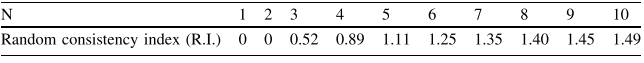
\includegraphics[scale = 0.9]{img/RI.png}
	\quelle{\cite[S.9]{Saaty.2012}}
	\caption{Durchschnittlicher RI nach Saaty}
	\label{img:ri2}
\end{figure}\\
Saaty stellt für den \ac{RI} eine eigene nach n geordnete Tabelle zur Verfügung. Für n=6 ist der \ac{RI} 1,25. Dadurch ergibt sich für die Matrix \ref{all}: 
\[CR=\frac{\mbox{\ac{CIx}}}{\mbox{\ac{RI}}}=\frac{0,107}{1,25}=0,0856\]
Es ergibt sich ein \ac{CR} von 0,0856. Dieser liegt unter der von Saaty definierten Grenzen von 0,0856 < 0,10. Die Matrix entspricht also nur 8,56\% einer zufällig verteilten Matrix und liegt damit im Rahmen. Die Matrix ist konsistent genug, um weiter fortzufahren.
\subsection{Gewichtung der Alternativen}
Nachdem die Alternativen gewichtet und diese Gewichtungen geprüft wurden, können nun die Alternativen bewertet werden. Nicht quantitativ messbare Bewertungen wurden in Absprache mit der Abteilung getroffen. Dabei werden die Bewertungen kurz erklärt, und es wird auf Besonderheiten beziehungsweise auffällige Merkmale hingewiesen. Jede einzelne Bewertung kann allerdings nicht erklärt werden, da dies zu ausufernd ist.
\subsubsection{Kosten}
\begin{table}[h!]
	\ra{1.5}
	\centering
	\begin{tabular}{c|cccc}
		monatliche Kosten   & Jenkins CI		 & Travis CI& Circle CI & GitLab CI   \\ 
		\hline
		Jenkins CI      & 1     		      &        9        &      9       &      2     \\
		Travis CI &   $\frac{1}{9}$     & 1               &  2&$\frac{1}{7}$      \\
		Circle CI   &   $\frac{1}{9}$     &  $\frac{1}{2}$   & 1            & $\frac{1}{8}$  \\
		GitLab CI    &    $\frac{1}{2}$    &  7   &        8      & 1           \\
	\end{tabular}
	\caption{Gewichtungsmatrix der monatlichen Kosten}
	\label{moncost}
\end{table}
In \ref{moncost} ist die Bewertung aller Kriterien im Vergleich zueinander zu finden im Hinblick auf die monatlichen Kosten. Es werden die monatlichen Preise für selbstgehostete Instanzen verglichen. Dabei werden die Serverkosten aus der Gleichung gestrichen, weil alle Tools auf derselben Hardware laufen würden. Aus diesem Grund sind die Serverkosten für diesen Vergleich zu vernachlässigen. Des Weiteren wird der Preis in Kosten pro 20 Usern verglichen, um eine Vergleichbarkeit herzustellen. Denn Circle CI bietet eine Lizenz zum Eigenhosting erst ab 20 Usern an. Somit kommt man auf Kosten von jeweils:
\begin{itemize}
	\item \textbf{Jenkins CI} 0 US-Dollar
	\item \textbf{Travis CI} 666 US-Dollar
	\item \textbf{Circle CI} 700 US-Dollar
	\item \textbf{GitLab CI} 80 US-Dollar
\end{itemize}
GitLab bietet zwar auch eine kostenfreie Version an, allerdings beinhaltet diese nicht viele Möglichkeit der Administration. Aus diesem Grund ist man in diesem Fall gezwungen, das \enquote{Starter}-Paket zu kaufen. Dort ist die Administration deutlich erweitert. Diese monatlichen Kosten werden nun in in Werte auf der Saaty Skala von 1-9 umgewandelt. Dabei wird der größte Wert im Vergleich zu dem niedrigsten Wert auf 9 gesetzt. Indem man diesen Wert durch 9 dividiert, erhält man 9 Abstufungen, durch die, die anderen Alternativen bewertet werden können.
\begin{table}[h!]
	\ra{1.5}
	\centering
	\begin{tabular}{c|cccc}
		initiale Kosten   & Jenkins CI		 & Travis CI& Circle CI & GitLab CI   \\ 
		\hline
		Jenkins CI      & 1     		      &        2       &      3      &      1     \\
		Travis CI &    $\frac{1}{2}$    & 1               &  2&$\frac{1}{3}$      \\
		Circle CI   &   $\frac{1}{3}$     &  $\frac{1}{2}$   & 1            & $\frac{1}{4}$  \\
		GitLab CI    &    1   &  3   &        4      & 1           \\
	\end{tabular}
	\caption{Gewichtungsmatrix der initialen Kosten}
	\label{icost}
\end{table}\\
Als Nächstes sind die initialen Kosten zu bewerten. Da kein Tool eine initiale Pauschale verlangt, wird dabei vorrangig auf den Arbeitsaufwand bei der Einrichtung der Tools geachtet. Denn der Mitarbeiter, der die Tools einrichtet, verursacht natürlich auch Kosten. Somit findet die Bewertung im Kontext des Arbeitsaufwandes statt.\\
 Das Ergebnis ist in \ref{icost} zu sehen. GitLab und Jenkins erhalten relativ viele Punkte dadurch, dass sie einfach einzurichten sind. Allerdings zeigt sich durch die geringen Unterschiede bei der Höhe der Bewertung, dass alle Tools ohne großen Aufwand einzurichten sind.
\subsubsection{Erweiterbarkeit}
\begin{table}[h!]
	\ra{1.5}
	\centering
	\begin{tabular}{c|cccc}
		Anbindung  & Jenkins CI		 & Travis CI& Circle CI & GitLab CI   \\ 
		\hline
		Jenkins CI      & 1     		      &        4        &      6       &      7     \\
		Travis CI &   $\frac{1}{4}$     & 1               &  3& 5     \\
		Circle CI   &   $\frac{1}{6}$     &  $\frac{1}{3}$   & 1            & 2  \\
		GitLab CI    &    $\frac{1}{7}$    &  $\frac{1}{5}$   &  $\frac{1}{2}$ & 1           \\
	\end{tabular}
	\caption{Gewichtungsmatrix der Anbindung}
\end{table}
Bei der Anbindung der Tools geht es sowohl um die Inputs als auch um die Outputs der Tools. Bei den Inputs geht es vorangig um die Anbindung an verschiedene Quellsysteme. Jenkins CI bietet praktisch für jedes VCS (siehe \ref{vcs}) ein Plugin an, um dieses einbinden zu können. Andersrum beschränkt sich Travis CI auf einen einzigen Hoster des VCS Git: Github. GitLab hat auch nur die Möglichkeit, das eingebaute VCS zu nutzen. Gegen einen Aufpreis ist es aber möglich, auch GitHub anzubinden.\\
Die Outputs von \ac{CI}/\ac{CDE}/\ac{CD}-Tools können sehr vielfältig sein. Dabei geht es zum einen um den tatsächlichen Output von compiliertem Code und deren Deploymentmöglichkeiten und zum anderen um die Nachrichtenkanäle, die von dem Tool bedient werden können. Bei der Anzahl der Deploymentmöglichkeiten liegt Jenkins CI wieder deutlich vorne. Durch die große Zahl an Plugins gibt es eigentlich für jedes System, sei es OnPremise oder in der Cloud, eine Möglichkeit Applikationen zu deployen. Alle anderen Tools fokussieren sich mehr auf die Cloud. Allerdings bieten sie meistens noch eine Möglichkeit, über eine Direktverbindung eine Applikation auf dem Zielsystem zu deployen. Dabei ist der Aufwand allerdings höher.\\
Bei den Nachrichtenkanälen bieten alle Systeme eigentlich den gleichen Umfang. Alle integrieren die meisten gängigen Chatprogramme und natürlich E-Mail.
\begin{table}[h!]
	\ra{1.5}
	\centering
	\begin{tabular}{c|cccc}
		Art der Software   & Jenkins CI		 & Travis CI& Circle CI & GitLab CI   \\ 
		\hline
		Jenkins CI      & 1     		      &       5       &     5      &      1    \\
		Travis CI &   $\frac{1}{5}$     & 1               &  1&$\frac{1}{5}$      \\
		Circle CI   &   $\frac{1}{5}$     &  1   & 1            & $\frac{1}{5}$  \\
		GitLab CI    &    1 		 &  5   &        5      & 1           \\
	\end{tabular}
	\caption{Gewichtungsmatrix der Art der Software}
\end{table}\\
Die Art der Software ist relativ schwierig zu bewerten. Wie bei der Beschreibung des Kriteriums bereits erwähnt, ist es schwierig zu bewerten, welche Art von Software in diesem Fall besser ist. Da aber Support als Extrakriterium ausgelagert wurde, kann Open Source als bessere Alternative angesehen werden. Sowohl Jenkins CI als auch GitLab bieten ihren Code quelloffen an. Somit werden diese beiden höher bewertet mit jeweils einer 5.
\subsubsection{Flexibilität}
\begin{table}[h!]
	\ra{1.5}
	\centering
	\begin{tabular}{c|cccc}
		Flexibilität   & Jenkins CI		 & Travis CI& Circle CI & GitLab CI   \\ 
		\hline
		Jenkins CI      & 1     		      &        9        &      9       &      5     \\
		Travis CI &   $\frac{1}{9}$     & 1               &  3&$\frac{1}{5}$      \\
		Circle CI   &   $\frac{1}{9}$     &  $\frac{1}{3}$   & 1            & $\frac{1}{7}$  \\
		GitLab CI    &    $\frac{1}{5}$    &  5   &       7      & 1           \\
	\end{tabular}
	\caption{Gewichtungsmatrix der Flexibilität}
\end{table}
Bei der Flexibilität kommt es auf die Anzahl der möglichen Zielsysteme an. Zielsysteme sind dabei die Plattformen, auf denen die Tools installiert werden können. Je größer die Anzahl, desto  flexibler ist das Tool einsetzbar. So ist Jenkins zum Beispiel auf jeder Plattform mit einer Java Installation verfügbar, unabhängig vom Betriebssystem. Das komplette Gegenteil dazu ist zum Beispiel Travis CI, welches nur auf Ubuntu 16.04, einer Linux Distribution, läuft. Circle CI kann darüber hinaus nur in der Cloud bei Amazon Web Services (AWS) installiert werden. GitLab bietet Versionen für viele Linux Betriebssysteme an, allerdings nicht für Windows. Außerdem können sowohl Jenkins als auch GitLab in einem Docker Container betrieben werden.
\subsubsection{Performance}
\begin{table}[h!]
	\ra{1.5}
	\centering
	\begin{tabular}{c|cccc}
		Performance   & Jenkins CI		 & Travis CI& Circle CI & GitLab CI   \\ 
		\hline
		Jenkins CI      & 1     		      &        1       &     1       &     1     \\
		Travis CI &   1   & 1               &  1&1     \\
		Circle CI   &  1   & 1   & 1            & 1  \\
		GitLab CI    &   1    &  1  &      1      & 1           \\
	\end{tabular}
	\caption{Gewichtungsmatrix der Performance}
\end{table}
Die Performance ist nur schwer vergleichbar zu bewerten, da die zugrundeliegende Hardware einen großen Teil der Performance ausmacht. Außerdem bieten alle Tools die Möglichkeit, die arbeitsintensive Prozesse auf andere Systeme auszulagern und so die Performance zu steigern. Aus diesem Grund werden alle Tools gleich bewertet. Es gibt keine signifikanten Unterschiede.
\subsubsection{Zuverlässigkeit}
\begin{table}[h!]
	\ra{1.5}
	\centering
	\begin{tabular}{c|cccc}
		Support   & Jenkins CI		 & Travis CI& Circle CI & GitLab CI   \\ 
		\hline
		Jenkins CI      & 1     	&  $\frac{1}{7}$        &      $\frac{1}{7}$       &      $\frac{1}{5}$     \\
		Travis CI &  7    & 1         &  1  	&   3      \\
		Circle CI   &   7    &  1 & 1            & 3  \\
		GitLab CI    &    5   &  $\frac{1}{3}$   &    $\frac{1}{3}$   	& 1           \\
	\end{tabular}
	\caption{Gewichtungsmatrix des Support}
\end{table}
Der Support kann sowohl an der Erreichbarkeit als auch an dem Umfang gemessen werden. Bei Jenkins gibt es keinerlei erreichbaren Support, da es sich um ein von einer Community entwickeltem Tool handelt. Alle anderen stellen einen Support zur Verfügung. Dabei kommt es bei GitLab allerdings darauf an, welches Paket man gekauft hat. Erst bei den teuersten Paketen ist auch 24-Stunden-Support inbegriffen. Ansonsten ist nur ein \enquote{Next-Day Support} vorgesehen. Travis CI und Circle CI bieten ähnliche Pakete an. Was alle gemeinsam haben, ist eine gut geschriebene und übersichtliche Dokumentation, unter anderem auch von häufig auftretenden Fehler, so dass diese schnell selber gelöst werden können.
\begin{table}[h!]
	\ra{1.5}
	\centering
	\begin{tabular}{c|cccc}
		Erreichbarkeit   & Jenkins CI		 & Travis CI& Circle CI & GitLab CI   \\ 
		\hline
		Jenkins CI      & 1     		      &        2       &      1       &      3     \\
		Travis CI &   $\frac{1}{2}$     & 1               &  $\frac{1}{2}$&2      \\
		Circle CI   &   1    &  2  & 1            & 3  \\
		GitLab CI    &    $\frac{1}{3}$    &  $\frac{1}{2}$   &        $\frac{1}{3}$     & 1           \\
	\end{tabular}
	\caption{Gewichtungsmatrix der Erreichbarkeit}
\end{table}\\
Die tatsächliche Erreichbarkeit eines Systems, ist ohne dass das System bereits im Einsatz ist, schwer zu bestimmen. Deswegen werden die folgenden Bewertungen aus den Systemen der Hersteller errechnet. Allerdings ist die Aussagekraft dieser Zahlen anzuzweifeln, da die meisten Fehler nicht durch die Tools selber verursacht werden, sondern durch die zugrundeliegende Hardware oder andere Subsysteme. Für die Bewertung wurden die Downtimes der letzten Tage aller Systeme verglichen und anschließend bewertet. Aufgrund der oben genannten geringen Aussagekraft werden die Spannen in den Bewertungen selbst klein ausfallen.  
\subsubsection{Sicherheit}
\begin{table}[h!]
	\ra{1.5}
	\centering
	\begin{tabular}{c|cccc}
		Sicherheit   & Jenkins CI		 & Travis CI& Circle CI & GitLab CI   \\ 
		\hline
		Jenkins CI      & 1     		      &        2       &      2     &     2      \\
		Travis CI &   $\frac{1}{2}$  & 1               &       1      &      1      \\
		Circle CI   &   $\frac{1}{2}$    &  1  & 1            &       1      \\
		GitLab CI    &    $\frac{1}{2}$    &  1   &        1      & 1           \\
	\end{tabular}
	\caption{Gewichtungsmatrix der Sicherheit}
	\label{safe}
\end{table}
Die Bewertung der Alternativen im Hinblick auf die Sicherheit ist in den vier Fällen recht einfach zu treffen. Alle Tools benutzten dieselben Sicherheitsprotokolle und Verschlüsselungen. Alle bieten die Möglichkeit, den Traffic sowohl zwischen der Weboberfläche und dem Server als auch zwischen dem Server und den Slaves mithilfe von TLS zu verschlüsseln. Somit geht es bei der Bewertung vorrangig um Extras wie zum Beispiel ein Credential Store bei Jenkins CI, um Zugangsdaten sicher im System hinterlegen zu können.
\subsection{Berechnung der Gesamtgewichtung}
Um die abschließende Reihenfolge der Alternativen bilden zu können, müssen die lokalen Prioritäten der einzelnen Alternativen im Bezug auf die Kriterien gebildet werden. Diese werde auf die gleiche Weise wie die Gewichtungen der Kriterien gebildet. In \ref{weight} sind alle errechneten Prioritäten zu sehen.
\begin{table}[h!]
	\ra{1.5}
	\centering
	\begin{tabular}{c|ccccc}
			 & mon. Kosten		& i. Kosten	 & Anbindung & Art der Software & Flexibilität   \\  
		\hline
		Jenkins CI   & 0,539    &        0,336        &      0,6       &      0,416   & 0,632 \\
		Travis CI &   0,066     & 0,164           &  0,24			&0,083 &  0,081  \\
		Circle CI   &   0,045    &  0,097   & 0,098           & 0,083 & 0,043\\
		GitLab CI    &    0,349   &  0,4 		  &        0,06      & 0,416        & 0,243 \\
	\end{tabular}
	\begin{tabular}{c|ccccc}
			&	Performance & Support & Erreichbarkeit &Sicherheit\\  
		\hline
		Jenkins CI      & 0,25  &        0,048    & 0,35    &  0,4  \\
		Travis CI &   0,25     & 0,393        &   0,189   &  0,2 \\
		Circle CI   &   0,25     &  0,393   &  0,35  &0,2 \\
		GitLab CI    &   0,25    &  0,164     &   0,109  & 0,2  \\
	\end{tabular}
	\caption{Zusammengefasste Gewichtungen aller Kriterien}
	\label{weight}
\end{table}\\
Da es sich aber nur um lokale Prioritäten handelt, müssen diese noch mit den globalen Prioritäten der Kriterien multipliziert werden. Dadurch ergeben sich die globalen Prioritäten der Bewertungen der Alternativen. Durch das Summieren ergibt sich die abschließende Reihenfolge der Alternativen.
\begin{table}[h!]
	\ra{1.5}
	\centering
	\begin{tabular}{c|ccccc}
		& mon. Kosten		& i. Kosten	 & Anbindung & Art der Software & Flexibilität   \\  
		\hline
		Gewicht.   & 0,238    &    0,08        &      0,071      &      0,015   & 0,025 \\
		\hline
		Jenkins CI   & 0,128    &        0,026        &      0,042       &      0,006   & 0,015 \\
		Travis CI &   0,015     & 0,013           &  0,017				&0,001 &   0,002 \\
		Circle CI   &   0,01    &  0,007   		 & 0,007         		& 0,001 & 0,001\\
		GitLab CI    &    0,083   &  0,032 		  &        0,004      & 0,006        & 0,006 \\
	\end{tabular}
	\begin{tabular}{c|cccc|c}
		&	Performance & Support & Erreichbarkeit &Sicherheit&Prioritäten\\  
		\hline
		Gewicht.      & 0,046  &        0,046    & 0,184   &  0,293 & \\
		\hline
		Jenkins CI      & 0,015  &        0,002    & 0,064   &  0,117 &0,415 \\
		Travis CI &   0,015    & 0,018        &   0,034   &  0,058 &0,172\\
		Circle CI   &   0,015     &  0,018   &  0,064  &0,058 &0,18\\
		GitLab CI    &   0,015    &  0,007     &   0,02  & 0,058 &0,229 \\
	\end{tabular}
	\caption{Zusammengefasste Gewichtungen aller Kriterien mit Summe}
	\label{weight2}
\end{table}\\
In \ref{weight2} ist die komplette Berechnung zu finden. Die abschließende Reihenfolge lautet wie folgt:
\begin{itemize}
	\item \textbf{1: Jenkins CI} \enspace\dotfill\enspace 0,415\enspace\enspace\enspace
	\item \textbf{2: GitLab CI} \enspace\dotfill\enspace 0,229\enspace\enspace\enspace
	\item \textbf{3: Circle CI} \enspace\dotfill\enspace 0,18\enspace\enspace\enspace
	\item \textbf{4: Travis CI} \enspace\dotfill\enspace 0,172\enspace\enspace\enspace
\end{itemize}
Es zeigt sich deutlich, dass Jenkins CI als beste Alternative aus dieser Analyse hervorgeht. Mit 0,415 liegt Jenkins CI 0,186 vor der nächsten Alternative, GitLab, auf dem zweiten Platz. Das ist ein sehr deutlicher Vorsprung ,der zeigt, dass Jenkins CI den anderen Alternativen deutlich überlegen ist. Besonders im Bereich der Kosten kann sich Jenkins CI behaupten. Um die Ergebnisse auf ihre \enquote{Robustheit} zu testen, wird nun noch eine Sensitivittsanalyse durchgeführt. Sie testet die Veränderung der Ergebnisse bei Veränderung an den Gewichtungen der Kriterien.\\ \\
\begin{table}[h!]
	\ra{1.5}
	\centering
	\begin{tabular}{c|ccccc}
		& mon. Kosten		& i. Kosten	 & Anbindung & Art der Software & Flexibilität   \\  
		\hline
		Gewicht.   &$\frac{1}{9}$    & $\frac{1}{9}$       &  $\frac{1}{9}$      & $\frac{1}{9}$  &$\frac{1}{9}$ \\
		\hline
		Jenkins CI   & 0,059    &      0,037      &      0,066      &      0,046   & 0,070 \\
		Travis CI &   0,007     & 0,018          &  0,026				&0,009 &   0,009 \\
		Circle CI   &   0,005    &  0,01   		 & 0,01         		& 0,009 & 0,004\\
		GitLab CI    &    0,038   &  0,044 		  &        0,006     & 0,046        & 0,027 \\
	\end{tabular}
	\begin{tabular}{c|cccc|c}
		&	Performance & Support & Erreichbarkeit &Sicherheit&Prioritäten\\  
		\hline
		Gewicht.      & $\frac{1}{9}$  &    $\frac{1}{9}$  & $\frac{1}{9}$ & $\frac{1}{9}$ & \\
		\hline
		Jenkins CI      & 0,027 &        0,005    & 0,038   &  0,044 &0,397 \\
		Travis CI &   0,027    & 0,043        &   0,021   &  0,022 &0,185\\
		Circle CI   &   0,027     &  0,043   &  0,038  &0,022 &0,173\\
		GitLab CI    &   0,027    &  0,018     &   0,012  & 0,022 &0,243 \\
	\end{tabular}
	\caption{Gewichtungsmatrix der Sensitivitätsanalyse}
	\label{weight3}
\end{table}\\
In \ref{weight3} wurde die Sensitivitätsanalyse durchgeführt. Dabei wurden alle Gewichtungen gleich verteilt. Jede Gewichtung beträgt $\frac{1}{9}$. Somit hat die Bewertung der Alternativen einen viel höheren Einfluss auf das Gesamtergebnis. Trotz dieser Veränderung ist Jenkins CI weiterhin auf dem ersten Platz. Lediglich die Plätze 3 und 4 haben getauscht. Travis CI ist bei dieser Verteilung einen Platz aufgestiegen. Ansonsten hat sich im Gegensatz zum Ausgangsergebnis nicht viel getan.\\
Durch dieses klare Ergebnis kann die Sensitivitätsanalyse an diesem Punkt abgebrochen werden. Normalerweise würde noch der \enquote{Break-Event-Punkt} berechnet werden. Das ist der Punkt, an dem die Reihenfolge der ersten Plätze sich verändert. Allerdings hat Jenkis CI einen solch großen Abstand auf die anderen Alternativen, dass es sich nicht lohnt, diesen zu berechnen. Somit ist die erste berechnete Reihenfolge auch die Abschließende.
\section{Handlungsempfehlung}
Die AHP-Analyse hat ergeben, dass Jenkins die beste Alternative im Vergleich zu Travis CI, Circle CI und GitLab CI ist. Aber ist dies auch die tatsächlich beste Alternative im Hinblick auf alle Faktoren, auch jene, die nicht in der AHP-Analyse aufgetaucht sind? Im Folgenden wird dies noch einmal diskutiert, um der Abteilung eine Handlungsempfehlung auszusprechen. Diese bezieht sich auf die Problemstellung aus der Einleitung.\\
Laut der AHP-Analyse wäre Jenkins CI also das beste Tool, um \ac{CI}/\ac{CDE}/\ac{CD} as a Service anzubieten. Dieser Meinung ist auch der Autor dieser Arbeit. Aufgrund reichlicher Vorerfahrung in der Arbeit mit Jenkins CI wäre er zu dem gleichen Ergebnis gekommen. Durch die Quelloffenheit, dem großen Angebot an Plugins und den nicht existenten Kosten ist Jenkins CI den anderen Tools in diesem Anwendungsfall deutlich überlegen. Besonders der Kostenfaktor macht einen großen Unterschied. Die Konfiguration ist dabei ein wenig aufwendiger als bei den anderen Tools, allerdings lässt sich Jenkins CI auch deutlich umfangreicher konfigurieren. Es werden dafür nur die nötigen Kompetenzen in der Abteilung benötigt. Diese sind allerdings durch vorherige Entwicklungsprojekte mit Jenkins Ci als \ac{CI}/\ac{CDE}/\ac{CD}-Tool bereits vorhanden.\\
Somit ist die deutliche Handlungsempfehlung dieser Arbeit, dass Jenkins CI für das \ac{CI}/\ac{CDE}/\ac{CD} as a Service Angebot genutzt wird. 
\chapter{Zusammenfassung}
In diesem Kapitel wird die Arbeit noch einmal rekapituliert und zusammengefasst. Es findet die Evaluation des Erkenntnisgewinns sowie eine kritische Reflexion der Ergebnisse statt. Es wird außerdem ein Ausblick auf eine mögliche Implementierung gegeben.
\section{Fazit}
Ziel dieser Arbeit war es, ein \ac{CI}/\ac{CDE}/\ac{CD}-Tool für die Nutzung als \ac{CI}/\ac{CDE}/\ac{CD} as a Service zu evaluieren. Dafür wurden zuerst die informationstechnischen Grundlagen geschaffen, indem Continuous Practices und Versionsverwaltungssysteme vorgestellt wurden. Darüber hinaus wurden drei vergleichende Analysemethoden evaluiert. Dabei wurde die AHP-Analyse als beste Methode für die spätere Analyse ausgewählt und nochmal im Detail beschrieben.\\ Anschließend wurden zusammen mit der Abteilung sowohl technische Alternativen als auch Vergleichskriterien erarbeitet. Als technische Alternativen wurden Jenkins CI, Travis CI, Circle CI und GitLab CI ausgewählt und kurz vorgestellt. Des Weiteren wurden neun Vergleichskriterien erarbeitet, anhand derer die vier Alternativen verglichen wurden. Dazu wurden zuerst die Kriterien gewichtet, um im weiteren Verlauf die Alternativen erst zu bewerten und dann mit den Gewichtungen der Kriterien zu verrechnen. Daraus ergab sich die folgende Reihenfolge der Alternativen:
\begin{itemize}
	\item \textbf{1: Jenkins CI} \enspace\dotfill\enspace 0,415\enspace\enspace\enspace
	\item \textbf{2: GitLab CI} \enspace\dotfill\enspace 0,229\enspace\enspace\enspace
	\item \textbf{3: Circle CI} \enspace\dotfill\enspace 0,18\enspace\enspace\enspace
	\item \textbf{4: Travis CI} \enspace\dotfill\enspace 0,172\enspace\enspace\enspace
\end{itemize}
Jenkins CI geht daraus deutlich als beste Alternative hervor. Deswegen sagt auch die Handlungsempfehlung dieser Arbeit aus, dass Jenkins CI die beste Alternative für die Implementierung als \ac{CI}/\ac{CDE}/\ac{CD} as a Service ist.\\ Die Ergebnisse dieser Arbeit wurden der Abteilung vorgestellt. Dort wurde das Ergebnis positiv aufgenommen aufgrund der Vorkenntnisse mit Jenkins CI. Trotz dieses Vorwissens bringt diese Arbeit ein Erkenntnisgewinn für die Mitarbeiter der Abteilung. Viele von ihnen hatten entweder noch kein Wissen mit \ac{CI}/\ac{CDE}/\ac{CD} gesammelt oder konnten die verschiedenen Practices nicht voneinander trennen. Mithilfe dieser Arbeit konnte ein einheitlicher Wissensstand innerhalb der Abteilung geschaffen werden. Mit der Arbeit wurde außerdem die Grundlage für das weitere Vorgehen mit \ac{CI}/\ac{CDE}/\ac{CD} as a Service gegeben. Vor dieser Arbeit war nur die Idee vorhanden. Damit ist der erste Schritt in Richtung einer erfolgversprechenden Implementierung des Service getan. 
\section{Kritische Reflexion}
Am Ende dieser Arbeit steht allerdings trotzdem noch kein Prototyp eines Service beziehungsweise keine Planung für die tatsächliche Implementierung. Es fehlte an Zeit für eine Ausarbeitung. Die Evaluierung der Tools hat die meiste Zeit eingenommen und keinen Raum für eine Ausarbeitung des Service gelassen. Dabei stellte die Analyse auch eine Herausforderung an sich dar. Es hat sich als schwierig herausgestellt, vergleichbare Kriterien zu finden. Wie man bei der Analyse gesehen hat, konnte bei dem Kriterium Performance keine Unterscheidung zwischen den Tool geschehen. Dies lag daran, dass die meisten Tools nicht implementiert werden konnten aufgrund von Lizenzkosten. Bei der Bewertung musste auf das Wissen der Abteilung zurückgegriffen werden. Durch die Einschränkung bei der Nutzung der Tools sollte auch das Ergebnis der AHP-Analyse kritisch betrachtet werden. Des Weiteren hatte Jenkins CI von Anfang an einen großen Vorteil durch die nicht vorhandenen Kosten zur Nutzung von Jenkins. Insgesamt kann man aber trotzdem sagen, dass die Arbeit eine positive Hilfe für die Abteilung ist.
\newpage
\section{Ausblick}
Dieser Teil der Arbeit wird genutzt, um einen Ausblick auf das mögliche weitere Vorgehen im Hinblick auf das Ergebnis der Arbeit zu geben. Dabei wird die Idee von \ac{CI}/\ac{CDE}/\ac{CD} as a Service weiter ausgereift.\\
Nachdem Jenkins CI als beste Alternative evaluiert wurde, wird der Service auf Jenkins aufsetzen. Dabei wird die Möglichkeit genutzt Jenkins in Docker zu betreiben. Das heißt, Jenkins wird nicht mehr lokal auf einem Server installiert, sondern es wird je nach Gebrauch ein Container mit einem Jenkins Docker Image gestartet. Dadurch ist Jenkins viel flexibler nutzbar. Wenn ein Kunde eine Jenkins Instanz bestellt ist es möglich, diese innerhalb weniger Minuten einsatzbereit zu haben. Es wird lediglich ein Hostsystem mit installiertem Dockerclient benötigt. Des Weiteren ist es sehr einfach möglich, Slavesysteme an den Jenkins anzubinden. Durch Docker ist es dem Jenkins Master möglich, so viele Slavesysteme wie benötigt werden hoch und auch wieder herunter zufahren. Dabei wird der Bedarf nach der Last, die auf dem System liegt, berechnet. Diese zusätzliche Rechenpower kann dem Kunden dann in Rechnung gestellt werden.
\begin{figure}[h!]
	\centering
	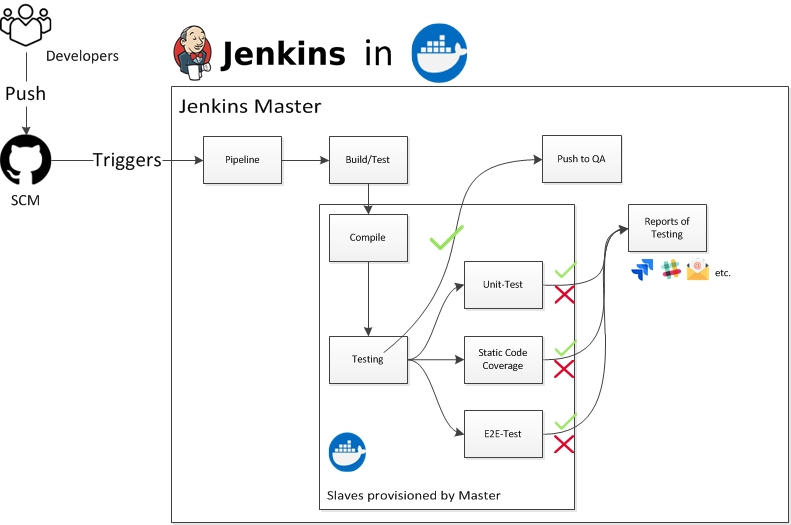
\includegraphics[scale = 0.7]{img/Jenkins.jpg}
	\caption{Ablauf Pipeline}
	\label{img:jenkins}
\end{figure}\\
In Abbildung \ref{img:jenkins} ist ein möglicher Ablauf einer Jenkinspipeline zu sehen. Zuerst werden die Veränderungen vom Entwicklerteam auf ein VCS-System gepusht. An Jenkins kann dabei jedes System von VCS angebunden werden. Diese Veränderung wird von Jenkins bemerkt und leitet den tatsächlichen Pipelineprozess ein. Dabei kommt nun der Knackpunkt mit den Slavessystemen. Für jeden Build und Test fährt Jenkins eigenständig Systeme hoch und lässt diese Prozesse einzeln laufen. Dadurch erhält jeder Test eine eigene \enquote{saubere} Umgebung. Sauber bedeutet in diesem Fall, dass keine Altdaten oder ähnliches auf den Systemen liegen und es somit zu keinen Interferenzen mit den Tests kommt. Am Ende werden die getesteten Applikationen automatisch auf den Zielsystemen deployt.\\
Wenn man die Idee mit vom \ac{CI}/\ac{CDE}/\ac{CD} as a Service weiter spinnt, bietet sich auch die Möglichkeit der automatischen Orchestrierung der einzelnen Jenkinscontainer an. Dadurch kann ein Kunde mit einem Knopfdruck seine Instanz erhalten. Das ist die Vision der Abteilung, und diese soll in naher Zukunft angegangenen werden und realisiert werden.